%% Los margenes, tipo de hoja y estilo BOOK
\documentclass[a4paper,11pt,twoside,openright,titlepage]{book}
\usepackage[utf8]{inputenc}
\usepackage{listings}
\usepackage{graphicx}
\usepackage{hyperref}
\usepackage{subcaption}
\usepackage{enumitem}
\usepackage{multicol}

\usepackage[nodisplayskipstretch]{setspace} \setstretch{1}
\let\oldv\verbatim
\def\verbatim{\par\setstretch{0.6}\oldv}

\setlength{\belowcaptionskip}{-8pt}


\usepackage[a4paper,left=1in,right=1in,top=0.6in]{geometry}

%\usepackage[T1]{fontenc}    %Ineterprete de tildes
%\usepackage[Latin1]{inputenc}
\usepackage{amsmath,amssymb}    %Paquete de entornos matematicos

\usepackage{natbib}
\usepackage[english,spanish]{babel}
%\selectlanguage{spanish}
\usepackage{graphicx}
\usepackage{psfrag}
%\usepackage{quotchap}
\usepackage{epsfig}
%\usepackage[all]{xy}

\usepackage{epsfig}
\usepackage{makeidx}
\usepackage{ifthen}
\usepackage{multicolpar}    %Para poner texto en columnas en plan articulo intercalado con texto normal
%\usepackage{multicol,multirow}

\usepackage{url}        %Para direcciones web
%\usepackage{marvosym}   %Para imprimir el simbolo de \EUR euro
%\usepackage{eurosym}   %Para imprimir el simbolo de \euro euro
\usepackage{fancybox}   %Para tablas con bordes redondeados


%% Modificacion de la plantilla para adaptarla a los requisitos de PFC
\usepackage{fancyhdr}
\pagestyle{fancy}
%%% Cabeceras y pies de pagina
\fancyhead[CE,CO]{\emph{\titulo}}
\fancyhead[LE,LO,RE,RO]{}
\fancyfoot[LE,RO]{\thepage}
\fancyfoot[CE,CO]{\leftmark}

\renewcommand{\footrulewidth}{.6pt}


%Definiciones de funciones para los titulos
\newlength\salto
\setlength{\salto}{3.5ex plus 1ex minus .2ex}

\newlength\resalto
\setlength{\resalto}{2.3ex plus.2ex}

\newcommand{\lsection}[1]
                {\section{#1}
                \vskip-.9\resalto   %%%% Aqui reculo el posible salto por defecto de \section
                \hrule
                \vskip+.9\salto}  %%%% vuelvo ha realizar el salto (puedes poner otra vez el 90%)


%Para imagenes de entornos estaticos \captionFigure{Texto Caption}{Texto Label}
\newcommand{\captionFigure}[2]{
    \refstepcounter{figure}
    \centerline{Figura \thefigure: #1 \label{#2}}
    \addcontentsline{lof}{section}{\thefigure.\ #1\label{#2}}
}

%Para imagenes de entornos estaticos \NOcaptionFigure{Texto Caption}{Texto Label} "No escribe el caption"
\newcommand{\NOcaptionFigure}[2]{
    \refstepcounter{figure}
    \addcontentsline{lof}{figure}{\thefigure.\ #1\label{#2}}
}


%% Datos del PFC
\newcommand{\titulo}{Herramientas modernas en redes neuronales: la librería keras}
\newcommand{\autor}{Autor: Carlos Antona Cortés}
\newcommand{\director}{Nombre Apellido1 Apellido2}
\newcommand{\tutor}{Tutor: José Ramón Dorronsoro Ibero}
%\newcommand{\ponente}{Ponente: Nombre Apellido1 Apellido2}
\newcommand{\vocal}{Nombre Apellido1 Apellido2}
\newcommand{\vocalsup}{Nombre Apellido1 Apellido2}
\newcommand{\presidente}{Nombre Apellido1 Apellido2}
\newcommand{\presidentesup}{Nombre Apellido1 Apellido2}
\newcommand{\fecha}{Enero 2017}
\newcommand{\carrera}{Grado en Ingenieria Informática}


\usepackage{color}
\usepackage{xcolor}
\usepackage{courier}
\usepackage{listingsutf8}
\lstset{
backgroundcolor=\color{white}, % choose the background color
basicstyle=\scriptsize\ttfamily, % size of fonts used for the code
breaklines=true, % automatic line breaking only at whitespace
captionpos=b, % sets the caption-position to bottom
commentstyle=\color{green}, % comment style
escapeinside={\%*}{*)}, % if you want to add LaTeX within your code
keywordstyle=\color{blue}, % keyword style
stringstyle=\color{magenta}, % string literal style
showstringspaces=false,
extendedchars=false,
inputencoding=utf8,
}


\begin{document}
\setlength{\baselineskip}{18pt}  %% Espacio interlinea
\setlength{\parskip}{6pt plus 1pt minus 1pt} %% Espacio interparrafo

\begin{titlepage}

\begin{center}

\vspace*{2cm}

\LARGE \textsc{Universidad Autónoma de Madrid}\\

\vspace{.2cm}

\large \textsc{Escuela politécnica superior}\\

\vspace{.2cm}

\begin{figure}[h]
    \begin{center}
        \begin{minipage}[c]{0.495\linewidth}
            \rightline{\epsfig{figure=images/logo_eps.eps,width=0.5\linewidth}}
        \end{minipage}
        \begin{minipage}[c]{0.495\linewidth}
            \leftline{\epsfig{figure=images/logo_uam.eps,width=0.5\linewidth}}
        \end{minipage}
    \end{center}
    \label{fig:Escudos}
\end{figure}

\Huge \carrera\\

\vspace{1cm}

\Huge \textsc{Trabajo Fin de Grado}\\

\vspace{1.5cm}

\Huge \MakeUppercase{\textbf{\titulo}}

\vspace{3cm}


\Large \autor\\
\Large \tutor\\
%\Large \ponente\\

\vspace{0.5cm}

\Large \fecha

\end{center}

\end{titlepage}

\normalsize


\newpage \thispagestyle{empty} % Pagina vacia


\frontmatter %Define el cuerpo inicial del libro en numeracion con letras romanas

\chapter*{}

\vspace*{0.2cm}

\begin{center}

\Huge \MakeUppercase{\textbf{\titulo}}

\vspace{7cm}

\Large \autor \\
\Large \tutor \\
%\Large \ponente \\

\vspace{5cm}


Codigo: 1617\_032\_CO \\
Dpto. de Neurocomputación \\
Escuela Politécnica Superior \\
Universidad Autónoma de Madrid \\
\fecha

\end{center}

\normalsize

\newpage \thispagestyle{empty} % Pagina vacia


\chapter*{Resumen}
El mundo de las redes neuronales está en auge. Poder simular el cerebro humano en un ordenador, parece ser uno de los hitos más prometedores de la informatica. Es cierto que este hito todavía no se ha conseguido, pero mediante algoritmos de machine learning, ya es posible entrenar máquinas para que aprendan de forma parecida a como lo haría nuestro cerebro. El objetivo de este Trabajo de Fin de Grado es poner en práctica estos algoritmos utilizando la librería Keras.\\\\
En primer lugar, se hará una breve introduccion al mundo de las redes neuronales. Se empezará por lo más básico, explicando que es una red neuronal y definiendo las partes mas importantes de su arquitectura. Una vez entendidos los conceptos básicos, se describirán los 3 tipos de redes neuronales mas extendidas actualmente debido a sus buenos resultados: Perceptrón multicapa, redes convolucionales, y redes LSTM.\\\\
En segundo lugar, se describirá Keras, una librería python de deep learning con la cual podremos diseñar nuestros propios modelos de redes neuronales. Se detallarán las clases y funciones más importantes, así como la gran cantidad de posibilidades que nos ofrece.\\\\
Por último, se aplicarán todos los conocimientos descritos anteriormente para diseñar cuatro tipos de redes neuronales que resolverán dos tipos de problemas distintos. En cuanto a problemas de clasificación de datos, veremos como clasificar distintas casas segun su precio a partir de cualidades que se han recogido previamente, y veremos como clasificacar imagenes en las que aparecen numeros, para determinar que numero es el que se representa en la imagen. Por otro lado, se llevarán a cabo dos problemas de predicción de datos. Mediante el primero, veremos como una maquina es capas de predecir si una persona tendrá diabetes a partir de sus datso médicos, y con el segundo, veremos como ésta es capaz de generar textos una vez haya sido entrenada con ellos.

\section*{Palabras Clave}
Redes neuronales, Keras, Tensorflow, perceptrón, redes convolucionales, redes LSTM, diabetes, housing, mnist, generador de texto.

\newpage
\chapter*{Abstract}
The world of neural networks is growing. Being able to simulate the human brain in a computer seems to be one of the most promising milestones in computing. It is true that it has not been achieved, but using machine learning algorithms, it is already possible to train machines to learn in a similar way as our brain. The objective of  this End-of-Grade Work is to implement these algorithms using the Keras library.\\
First of all, a brief introduction to the world of neural networks will be made. It will start with the basics, explaining what is a red neuron and defining the most important parts of its architecture. After understanding the basics, I will describe the three types of neural networks more rife due to their results: Multilayer Perceptron, Convolutional Networks, and LSTM Networks. \\\\
Secondly, I will describe Keras, a deep learning python library with which it is able to design our own neural network models. I will detail the classes and the most important functions, as well as the great amount of possibilities that this library offers us. \\\\
Finally, all previous knowledge is applied to design four types of neural networks that will solve two different types of problems. As for the problems of data classification, we will see how to classify several houses according to their price from qualities that have been previously collected, and we will see how to classify images of handwritten numbers, to determine which number is represented in the picture. On the other hand, data prediction problems will be addressed. Through the first example, we will be able to predict if a person will have diabetes or not analyzing their medical data, and with the second, we will see how a machine is able to generate texts once he has been trained with them.

\section*{Keywords}
Neural network, Keras, Tensorflow, perceptron, convolutional neural network, LSTM network, diabetes, housing, mnist, text generator.


\chapter*{Agradecimientos}
Antes de nada, quiero dar las gracias a mi tutor, José Dorronsoro por darme la oportunidad de adentrarme en el mundo de las redes neuronales. En una materia de estudio tan extensa, novedosa, y en constante desarrollo, me habría sido mucho mas dificil cumplir con mis objetivos si no fuese por su ayuda.\\\\
En segundo lugar quiero dar las gracias a mis compañeros de clase. Sergio, David, Javi, Galan, Gus, Alfonso... Durante estos 4 años han sido las personas a las que mas he visto, y por tanto, no pueden faltar en mis agradecimientos. Cuantos dias hemos pasado en las salas de estudio de la biblioteca, cuantas semanas quedandonos de principio a fin en la universidad estudiando, cuantas noches sin dormir lo que nos gustaría por entregar alguna practica... En fin, gracias por hacerme el camino mas ameno.\\\\
Una mención especial a mis amigos de Vallecas, Alvaro, Alberto, Ivan y Benze. En estos cuatro años hemos cambiado mucho, y gracias a las vacaciones, el canal de musica, las tardes de viernes en el bar... he conseguido tomarme ese respiro todas las semanas para abstraerme lo necesario de los estudios, y seguir disfrutando de la vida.\\\\
Por último, y no por ellos menos importante, quiero ofrecer una mención especial a mi familia. Ellos han sido los que verdaderamentre han tenido que aguantarme estos 19 años de estudio. Semanas de nervios, luces encendidas a altas horas de la noche, apoyos y consejos cuanto mas lo necesitaba... No tendría páginas suficientes en este TFG para agradecerles todo lo que han hecho por mi.

\tableofcontents

\newpage \thispagestyle{empty} % Pagina vacia

\addcontentsline{toc}{chapter}{Indice de Figuras}    %Para que aparezca en el indice
\renewcommand{\listfigurename}{Indice de Figuras}
\listoffigures

\newpage \thispagestyle{empty} % Pagina vacia

\addcontentsline{toc}{chapter}{Indice de Tablas}    %Para que aparezca en el indice
\renewcommand{\listtablename}{Indice de Tablas}
\listoftables

\newpage \thispagestyle{empty} % Pagina vacia

\mainmatter %Define el cuerpo principal del libro numeracion normal.

% \input{preambulo}

\chapter{Introducción}
\label{chap:intro}

\vspace{-0.2cm}

\lsection{¿Qué es deep learning?}
Deep Learning (aprendizaje profundo) es una rama de machine learning (aprendizaje automático) formada por un conjunto de algoritmos que intentan modelar abstracciones de alto nivel en datos, usando grafos profundos con múltiples capas de procesamiento. Estas capas de procesamiento pueden estar compuestas por transformaciones tanto lineales como no lineales.\\\\
Antes de entrar de lleno en este mundo tan complejo, relativamente moderno, y en constante cambio, no estaría de más entender que significa que una maquina pueda aprender. Muchas veces en el mundo de la informática, nos encontramos ante problemas que son difíciles de programar. Imaginemos el caso de una aplicación de reconocimiento de textos escritos a mano. Es difícil imaginarse un conjunto de reglas que permitan distinguir unos caracteres de otros, ya que dependiendo de la forma de escritura de cada individuo, los caracteres cambian relativamente su forma. Por ejemplo, podría ser bastante difícil distinguir el número 0 del numero 6 de la letra o. A parte de este ejemplo, también tenemos muchos tipos de problemas en los que cuesta imaginarse un conjunto de reglas para su resolución: reconocimiento de objetos, discursos... Aquí es donde entra en juego el Machine Learning en general, y el Deep Learning en partícular.\\\\
Si en vez de intentar escribir un programa que resuelva nuestro complejo problema, escribimos un algoritmo que permita a nuestro ordenador estudiar miles de ejemplos con sus soluciones, para luego aplicar la experiencia a la hora de resolver nuevos casos, estaremos aplicando Machine Learning.\\\\
El Deep Learning, que tuvo sus inicios en los años 80s, no es mas que un paradigma de implementación de Machine Learning. Debido a las recientes investigaciones sobre el mundo de la Inteligencia Artificial, esta tecnología se encuentra ahora mismo en constante desarrollo, ya que se ha demostrado que es la forma mas eficiente de hacer con un computador una simulación de lo que nuestro cerebro puede hacer.

\lsection{¿Qué podemos hacer mediante deep learning?}
TODO: De entrada, resolver problemas de clasificación y predicción...\\
Otros casos mas concretos podrían ser:
\textbf{1. Colorear imágenes en blanco y negro.}\\
Tradicionalmente, esta tarea ha sido llevada a cabo por el ser humano de manera manual, hasta que mediante el uso de deep learning, se han utilizado los objetos y contextos de las propias imágenes para ser coloreadas. Para ello, se necesitan grandes redes neuronales convolucionales con capas supervisadas, que recrean la imagen coloreada de la misma manera que lo haría un ser humano.\\
\\\textbf{2. Añadir sonido a películas mudas.}\\
Pongamos el ejemplo de querer recrear el sonido que hace un palo al golpear con una superficie. Si entrenamos el sistema utilizando una gran cantidad de vídeos donde se muestra el sonido que hace un palo al ser golpeado contra diferentes superficies, nuestra red neuronal asociará los frames del vídeo mudo con la información ya aprendida, y seleccionará el sonido que mejor se adapte a la escena.\\
\\\textbf{3. Traducciones automáticas.}\\
Pese a que la traducción de palabras, frases o textos lleva siendo posible desde hace muchos años, mediante la utilización de redes neuronales se han alcanzado resultados mucho mejores sobre todo en dos áreas: traducción de texto, y traducción de imágenes. En el caso de los textos por ejemplo, se ha pasado de traducir palabras sueltas, a analizar y entender la gramática y la conexión entre palabras, haciendo deducciones mucho mas precisas del significado global de la frase. Para ello, se usan redes LSTM. Para el caso de traducción de textos en imágenes se utilizan redes convoluciones, ya que son capaces de identificar letras, con ellas formar palabras, y a su vez formar un texto. En muchos contextos a esto se le llama traducción visual.\\
\\\textbf{4. Clasificación de objetos en fotografías.}\\
Esta funcionalidad consiste en detectar y clasificar uno o mas objetos de la escena de una fotografía. Eso se consigue entrenando grandes redes convolucionales mediante imágenes aisladas de objetos conocidos.\\
A partir de aquí, el siguiente punto es crear una palabra o frase que describa el contenido de la imagen. En 2014, hubo un "boom" de algoritmos que alcanzaron resultados impresionantes a la hora de resolver este problema. La mayoría de ellos usaban redes LSTM para convertir las etiquetas que se generan al detectar objetos en una imagen, en frases con sentido.\\
\\\textbf{5. Generación de textos.}\\
Esta tarea consiste en, dado una recopilación de textos, generar nuevos textos a partir de una palabra o una frase.\\
Una aplicación podría ser la generación de textos escritos a mano. La escritura a mano consiste en una serie de movimientos coordinados de un bolígrafo, en los que se crea texto. Mediante machine learning, podemos aprender la relación entre los movimientos del bolígrafo y las letras escritas, para generar nuevos ejemplos. Esta funcionalidad puede ser utilizada por médicos forenses, o especialistas en análisis de manuscritos, ya que es posible aprender una cantidad impresionante de estilos de escritura.\\
Otra posible aplicación sería la de generar nuevos textos con nuevas historias. Mediantes redes LSTM se ha conseguido aprender la relación entre los distintos elementos de un texto (letra, palabra, frase...), para después generar nuevos textos letra a letra o palabra a palabra. Los modelos son capaces de aprender como deletrear, puntuar, formar oraciones, e incluso copiar los estilos de escritura para generar dichos textos.\\
\\\textbf{6. Inteligencia artificial en videojuegos.}\\
Todos sabemos que la inteligencia artificial en los vídeos es una cosa que lleva existiendo desde hace mucho tiempo... En un shooter, la IA de la videoconsola sabe identificar donde está tu jugador, y con esa información, sabe a quien y donde disparar. Pero... ¿y si fuese posible analizar todos los píxeles de la pantalla? Mediante deep learning esto es relativamente sencillo, permitiendo a la IA rival tener mucha mas información y tomando así mejores decisiones. Un ejemplo nos lo encontramos en AlphaGo, una aplicación desarrollada por Google que ganó al campeón mundial de Go.\\\\
Otros ejemplos de aplicaciones de redes neuronales para resolver problemas actuales podrían ser: reconocimiento y traducción de discursos y charlas en tiempo real, foco automático en objetos en movimiento en fotografías, conversión automática de objetos en fotografías, respuestas automáticas a preguntas sobre objetos en fotografías... Como se puede observar, casi todas estas tareas se tratan de automatizar. Son tareas que el ser humano puede hacer manualmente, pero una maquina es capaz de aprender a hacerlo en mucho menos tiempo y con mucha mas eficiencia.




\lsection{Antecedentes y estado actual}

%\lsection{Motivación del proyecto}
%Ejemplo de referencia a la bibliografía~\cite{article:Ejemplo}.

%Ejemplo de imagen:
%\begin{figure}[h]
% \centerline{
%    \mbox{
\includegraphics[width=3.00in]{images/logo_eps.eps}}
%  }
%  \caption{Ejemplo pie de figura 1}
%  \label{fig:norm_Daugman}
%\end{figure}

%\lsection{Objetivos, enfoque, metodología y plan de trabajo}

\newpage \thispagestyle{empty} % Pagina vacia


\chapter{Redes neuronales: Deep Learning}
\lsection{Redes neuronales}
\subsection {Historia de las redes neuronales}
Las redes neuronales, como su nombre indica, pretenden imitar la forma de funcionamiento de las neuronas que forman el cerebro humano. 
\begin{itemize}
\item Entre los pioneros en el modelado de neuronas se encuentra Warren McCulloch y Walter Pitts, investigadores que propusieron un modelo matemático.
\item En 1949, Hebb definió dos conceptos muy importantes:
\begin{itemize}
\item El proceso de aprendizaje se localiza principalmente en la sinapsis o conexion entre neuronas.
\item La informacion se representa en el cerebro mediante un conjunto de neuronas activas o inactivas.
\end{itemize}
Estas dos reglas se sintetizan en la regla de aprendizaje de Hebb, que sigue siendo usada en los modelos actuales. Esta regla nos dice que los cambios en los pesos de la sinapsis se basan en la interacción entre las neuronas pre y post sintacticas, y el numero de veces que se activan de manera simultanea.
\item En 1956, en la ciudad de Dartmouth, se llevó a cabo la primera conferencia sobre Inteligencia Artificial donde se discutio sobre la capacidad de las maquinas para simular el aprendizaje humano.
\item En 1959, Widrow escribió la Teoria sobre la adaptacion neuronal, y desarrolló los Algoritmos Adaline (Adaptative Linear Neuron) y Madaline (Multiple Adaline). Con ellos, se consiguió llevar a cabo la primera aplicación de redes neuronales para solventar problemas reales: un filtro para eliminar ecos en las lineas telefonicas.
\item En 1962 Rosemblatt desarrolló el concepto de Perceptron. Esto dio lugar a la regla de aprendizaje Delta, que permitía emplear señales continuas de entrada y de salida. 
\item En 1984, Kohonen desarrolló una familia de redes de memoria asociativa y mapas auto-organizativos, actualemente llamadas redes de Kohonen.
\item Anderson desarrolló una red denominada Brain-State-in-a-Box, la cual trunca la salida lineal para que no se vuelva demasiado grande en las iteraciones de la red.
\item Grossberg y Carpenter desarrollaron las redes autoorganizativas de categorías ART (Teoria de la Resonancia Adaptativa)
\item Mediante las redes de Hopfield, se demostró que las redes asociativas pueden aprender por analogía a la autoorganizacion de los sistemas físicos.
\item Neocognitrón: Kinihiko Fukushima desarrolló una familia de redes para el reconocimiento de caracteres.
\item Mediante las máquinas de Boltzman se desarrolló la regla de aprendizaje basada en funciones de densidad de probabilidad.
\end{itemize}

\begin{figure}[htp]
\centering
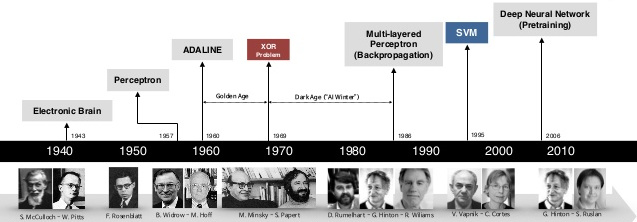
\includegraphics[scale=0.60]{images/history.jpg}
\caption{Historia de las redes neuronales}
\end{figure}

\subsection {La neurona biologica} \mbox{}\\
El cerebro, visto a un alto nivel y simplificando enormemente su estructura, podriamos decir que es un conjunto de millones y millones de celulas, llamadas neuronas, interconectadas entre ellas mediante sinapsis. La sinapsis se lleva a cabo en la zona donde 2 neuronas se conectan, y las partes de la célula que se encargan de realizarla son las dentritras y las ramificaciones del axón.
\begin{figure}[htp]
\centering
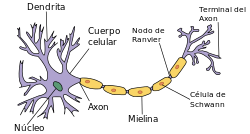
\includegraphics[scale=1]{images/neurona.png}
\caption{Estructura de una neurona}
\end{figure}\\
Cada neurona desarrolla impulsos eléctricos que se trasmiten a lo largo de esta mediante su axón. Este, al final se ramifica en ramificaciones axionales, que conectan con otras neuronas mediante sus dentritras.\\
El conjunto de elementos que hay entre la ramificacion axional y la dentrita forman la sinapsis, que regula la transmisión del impulso eléctrico mientre unos elementos químicos llamados neurotransmisores.
\begin{figure}[htp]
\centering
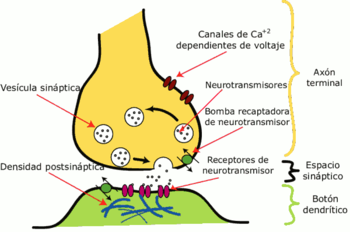
\includegraphics[scale=0.70]{images/sinapsis.png}
\caption{Sinapsis}
\end{figure}\\
Los neurotransmisones liberados en la sinapsis puedes tener un efecto negativo o positivo sobre la transmision del impulso eléctrico en la neurona que los recibe en sus dentritas. Esta neurona recibe varias señales de las distintas sinapsis, y las combina consiguiendo un cierto nivel de estimulacion. En función de de este nivel de activación, la neurona emite señales eléctricas mediante impulsos, con una intensidad determinada y con una frecuencia llamada tasa de disparo.\\
En resumen, si consideramos que la informacion del cerebro está codificada en impulsos eléctricos que se transmiten entre neuronas, y que los impulsos se ven modificados básicamente en la sinapsis, podemos intuir que la codificacion del aprendizaje estará en la sinapsis y en la forma en la que las neuronas dejan pasar o inhiben las señales segregando neurotransmisores.

\subsection {La neurona artificial} \mbox{}
Las neuronas artificiales son modelos que tratan de simular el comportamiento de las neuronas biológicas. Cada neurona se representa como una unidad de proceso que forma parte de una entidad mayor, la red neuronal.
\begin{figure}[htp]
\centering
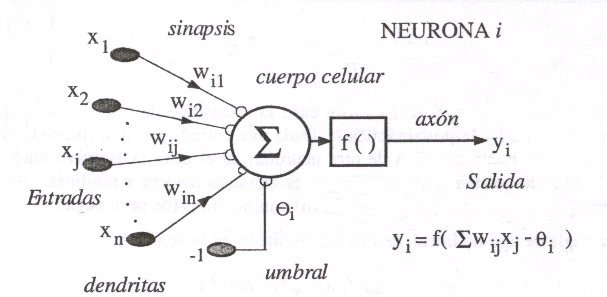
\includegraphics[scale=1]{images/neuronaartificial.jpg}
\caption{Esquema de una neurona artificial}
\end{figure}\\
Como podemos intuir observando la imagen anterior, la neurona aritifical se comporta como una biológica, pero de forma simplificada:
\begin{itemize}
\item Entradas (${x_{1}, x_{2}, x_{3}}$): estos valores pueden ser enteros, reales o binarios y equivaldrían a los impulsos que envian otras neuronas a través de sus dentritras.
\item Pesos (${w_{1}, w_{2}, w_{3}}$): equivaldrían a los mecanismos de sinapsis para transmitir el impulso. 
\item De este modo, la union de los valores ${x_{i} , w_{i}}$ equivaldría a las señales químicas inhibidoras y excitadoras que se dan en la neurona. Estos valores son la entrada de la funcion de activacion, que convierte todo el conjunto de valores en uno solo llamado potencial. La función de ponderación suele ser la suma ponderada de las entradas y los pesos sinápticos.
\item La salida de función de ponderación llega a la función de activación que transforma este valor en otro en el dominio que trabajen las salidas de las neuronas. Suele ser una función no lineal como la función paso o la función sigmoide, aunque también se usa funciones lineales.
\item El valor de salida cumpliría la función de la tasa de disparo en las neuronas biológicas. Suele ser la función identidad, aunque sistemas mas complejos no siguen esta regla.
\end{itemize}
En resumen:
\begin{itemize}
\item Neuronas biológicas $\Longleftrightarrow$ Neuronas Artificiales.
\item Conexiones sinápticas $\Longleftrightarrow$ Conexiones ponderadas.
\item Efectividad de las sinapsis$\Longleftrightarrow$ Peso de las conexiones.
\item Efecto excitador o inhibidor de una conexión $\Longleftrightarrow$ Signo del peso de una
conexión.
\item Activación $\rightarrow$ Tasa de disparo $\Longleftrightarrow$ Función de activación $\rightarrow$ Salida
\end{itemize}

\subsection {Funciones de las neuronas artificiales}
\subsubsection {Funcion de red o propagación}
Esta función se encarga de tranformar las diferentes entradas que provienen de la sinapsis, en el potencial de la neurona. Normalmente, las neuronas han de tratar simultaneamente con varios valores de entrada, y han de hacerlo como si se tratase de uno solo. Esta funcion viene a resolver el problema de combinar las entradas simples (${x_{1},x_{2},x_{3}...}$) en una sola entrada global. Podría describirme mediante la siguiente ecuación:
\begin{equation}
input = (x_{1}:w_{1})*(x_{2}:w_{2})*...*(x_{n}:w_{n})
\end{equation}
siendo ":" el operador apropiado (por ejemplo: máximo, sumatorio, producto...), "n" el numero de entradas y w el peso de las conexiones. Multiplicando las entradas por los pesos, se permite que un valo muy grande de entrada pueda tener una influencia pequeña, si sus pesos son pequeños.
\subsubsection {Funcion de activacion}
La funcion de activacion combina el potencial que nos proporciona la funcion de propagación con el estado actual de la neurona, para conseguir el estado futuro de esta (activada/desactivada). Esta funcion es normalmente creciente y monótona. Las funciones mas comunes son:
\begin{itemize}
\item Identidad: es una funcion de activacion muy simle que siempre devuelve como salida su valor de entrada. Su rango es va de menos infinito a infinito, es monotona y derivativamente monotona.
\begin{equation}
f(x) = x
\end{equation}
\begin{figure}[htp]
\centering
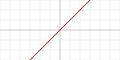
\includegraphics[scale=1]{images/Activation_identity.png}
\caption{Funcion de activación identidad}
\end{figure}
\item Escalón binario: Es la más usada por redes neuronales binarias ya que no es lineal, y es bastante sencilla. El Perceptron y Hopfield son algunos ejemplos de redes que usan esta funcion. Cuenta con un rango {0,1}, y es monótona.
\begin{equation}
f(x) = \begin{Bmatrix}
0 & x<0\\ 
1 & x\geq 0
\end{Bmatrix}
\end{equation}
\begin{figure}[htp]
\centering
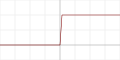
\includegraphics[scale=1]{images/Activation_binary_step.png}
\caption{Funcion de activación escalón binario}
\end{figure}
\item Logistica / Softstep: .............. Su rango va es (0,1), y es monótona.
\begin{equation}
f(x) = \frac{1}{1+e^{-x}}
\end{equation}
\begin{figure}[htp]
\centering
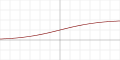
\includegraphics[scale=1]{images/Activation_logistic.png}
\caption{Funcion de activación logistica}
\end{figure}
\item Hiperbólica o tangencial: Esta funcion es utilizada por redes con salidas continuas. Un ejemplo sería el Perceptrón multicapa con retropropagación, ya que su algoritmo de aprendizaje necesita una función derivable. Cuenta con un rango (-1,1), es monótona, y se aproxima a la funcion identidad en su origen.
\begin{equation}
f(x) = \tanh(x) = \frac{2}{1+e^{-2x}}-1
\end{equation}
\begin{figure}[htp]
\centering
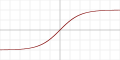
\includegraphics[scale=1]{images/Activation_tanh.png}
\caption{Funcion de activación tangencial}
\end{figure}
\item Rectificadora (ReLU): Esta funcion de activacion la introdujo por primera vez en el año 2000  Hahnloser, con motivaciones biológicas y matematicas. Se viene usando en redes convolucionales mas que la ampliamente extendida funcion logistica sigmoide (se basa en probabilidades), y es más practica que la tangente hiperbólica. La función rectificadora es, por tanto, una de las funciones de activacion más populares para deep learning.
\begin{figure}[htp]
\centering
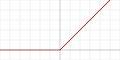
\includegraphics[scale=1]{images/Activation_rectified_linear.png}
\caption{Funcion de activación rectificadora}
\end{figure}
\item Softplus: aproximación suavizada de la funcion de activación rectificadora.
\begin{equation}
f(x) = ln(1+e^{x})
\end{equation}
\begin{figure}[htp]
\centering
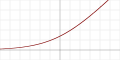
\includegraphics[scale=1]{images/Activation_softplus.png}
\caption{Funcion de activación softplus}
\end{figure}
\end{itemize}
Las propiedades deseables de una funcion de activación son:
\begin{itemize}
\item No lineal: Cuando contamos con una funcion de activación no lineal, se puede probar que una red neuronal de dos capas pueda ser una funcion universal de aproximacion. La funcion identidad no satisface esta propiedad, ya que si todas las capas utilizar la funcion de activacion identidad, la red neuronal entera equivaldría a un modelo con una sola capa.
\item Continuamente diferenciable: Esta propiedad es necesaria para que sean posibles los métodos de optimización basados en el gradiente. Por ejemplo, la funcion de activación de escalón binario no es diferenciable en el 0, y su derivada es 0 en todos los demas valores, asi que los metodos basados en el gradiente no funcionan con ella.
\item Rango: Cuando el rango de la funcion de activación es finito, los métodos de entrenamiento basados en gradiente tienden a ser mas estables porque los pesos a elegir son mas limitados. Cuando el rango es infinito, el entrenamiento es por lo general mas eficiente porque los patrones afectan mas a los pesos.
\item Monotona: Cuando la funcion de activación es monotona, el error en un modelo con una sola capa tiende a converger.
\item Suavidad: Las funciones con una derivación monotona tienden a ser mas generales en algunos casos.
\item Se aproxima a la funcion identidad cerca del origen: Cuando la función de activación tiene esta propiedad, la red neuronal aprende de forma mas eficiente cuando sus pesos son inicializados con valores pequeños aleatorios.
\end{itemize}

\subsubsection {Funcion de salida}
Esta función convierte el estado de la neurona en la salida hacia la siguiente. Recordar que esta salida es transmitida mediante la sinapsis. En ocasiones podemos encontrar redes neuronales sin funcion de salida, por lo que la salida es el propio estado de activación de la neurona. Nos encontramos dos grandes tipos de funciones de salidas.
\begin{itemize}
\item Funciones de salida que transforman el estado de activación en una salida binaria. Para ello, se utiliza la función escalón.
\item Funciones de salida que transforman el estado de activacion en probabilidades. Un ejemplo de uso nos lo encontramos en la máquina de Boltzman. Las redes con etse tipo de salidas no tiene un comportamiento determinista.
\end{itemize}


\subsection{Tipos de aprendizaje en redes neuronales}
\subsubsection {Aprendizaje supervisado} 
Cuando el problema nos presenta el conjunto de datos y los atributos que queremos precedir. Nos encontramos dos categorias:
\begin{itemize}
\item Regresion: los valores de salida son una o mas variables continuas. Un ejemplo sería predecir el valor de una casa en funcion de sus metros cuadrados, el numero de habitaciones, tamaño de la piscina...
\item Clasificación: los datos pertenecen a dos o mas clases, y queremos aprender como clasificar nuevas entradas en esas clases, a partir de datos que ya conocemos. Uno de los ejemplos más conocidos es el Iris dataset, donde se intenta clasificar los datos en 4 tipos de flores segun la longitud y la anchura de sus petalos y sépalos.
\end{itemize}
\subsubsection {Aprendizaje no supervisado} 
Cuando no hay informacion previa de salidas dado un conjunto de entradas. En estos casos, el objetivo es encontrar grupos mediante clustering, o determinar una distribución de probabilidad sobre un conjunto de entrada.



\section {Perceptron}
En 1959, F.Rosenblatt desarrolló por primera vez la idea de Perceptrón, basandose en la regla de aprendizaje de Hebb y en los modelos de neuronas biológicas de McCulloch y Pitts. Uno de las carácteristicas que mas interés despertó de este modelo fue su capacidad para aprender a reconocer patrones.\\
El perceptron se basa en una arquitectura monocapa. Está constituido por un conjunto de celulas de entrada, que reciben los patrones a reconocer o clasificar, y una o varias celulas de salida que se ocupa de clasificar estos patrones de entrada en clases. Cada célula de entrada está conectada con todas las células de salida. En la siguiente imagen se puede observar la arquitectura de un perceptron simple con 4 entradas y 1 salida.
\begin{figure}[htp]
\centering
\vspace{-1em}
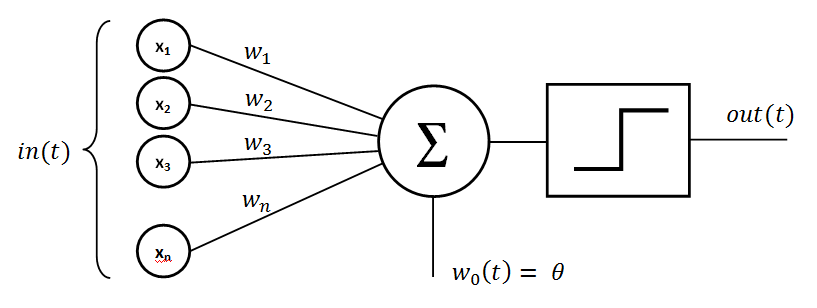
\includegraphics[scale=0.5]{images/perceptron.png}
\caption{Perceptron simple.}
\end{figure}
\\El umbral es un parámetro utilizado como factor de comparación a la hora de generar la salida. En esta arquitectura, la salida de la red se obtiene multiplicando los valores de las entradas, por los pesos de las conexiones:
\begin{equation}\label{Umbral perceptron}
y' =  \sum_{i=1}^{n} w_{i}x_{i}
\end{equation}
La salida definitiva se obtiene aplicandole la funcion de salida al nivel de activacion de la célula, es decir:
\begin{equation}\label{Salida perceptron}
y =  F(y', \theta)
\end{equation}
Con estas formulas, podemos deducir que la salida de la célula será 1 (neurona activada) si el umbral es mayor que 0, o 0 (neurona desactivada) en caso contrario.\\
La funcion de salida (F) produce una salida binaria, por lo que es un diferenciador en dos categorias. En el caso de tener unicamente dos dimensiones, la ecuación anterior se tranforma en:
\begin{equation}
w_{1}x_{1} + w_{2}x_{2} + \theta = 0
\end{equation}
Que es la ecuación de una recta con pendiente \begin{equation}-\frac{w_{1}}{w_{2}}\end{equation}, y cuyo corte en la abscina en el eje y pasa por \begin{equation}-\frac{\theta}{w_{2}}\end{equation}
Como podemos ver, podemos imaginarnos el percetron como una recta, que un gráfica de dos dimensiones, deja las dos categorías a separar a un lado y a otro de la misma.
\begin{figure}[htp]
\centering
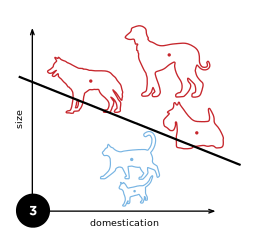
\includegraphics[scale=0.5]{images/Perceptron_example.png}
\caption{Separacion lineal del perceptrón.}
\end{figure}
\subsubsection{Aprendizaje}
El proceso de aprendizaje consiste en la inserción de un patrón de entrada del conjunto de aprendizaje perteneciente a la clase. Si la salida es correcta, no se realizará ninguna acciones, pero si no, se modificarán los pesos.
Para el perceptrón, existen 2 tipos de aprendizaje: uno utiliza una tasa de aprendizaje, mientras que el otro no la utiliza. Esta tasa de aprendizaje regula la actualización de los valores de los pesos de la red, y es la misma para todas las neuronas. Los pasos a seguir para entrenar el perceptrón son:
\begin{enumerate}
\item Inicialización de variables
\item Bucle de iteraciones:
\begin{enumerate}
\item Bucle para todos los ejemplos
\begin{enumerate}
\item Leer valores de entrada
\item Calcular error
\item Actualizar pesos segun el error
\begin{enumerate}
\item Actualizar pesos de entradas
\item Actualizarf el umbral
\end{enumerate}
\item Incremental contador de numero de ejemplos entrenados
\end{enumerate}
\item Comprobar que el vector de pesos es correcto
\item Incremental el contador de iteraciones
\end{enumerate}
\item Salida
\end{enumerate}

\subsubsection{Capacidades de un perceptron simple}
Hasta ahora, hemos descrito el perceptrón como un clasificador. Sin embargo, tambien pueden ser usados para emular funcines lógicas elementales como AND, OR y NAND. Consideremos las funciones AND y OR. Dado que son funciones linealmente separabales, pueden ser aprendidas por un perceptrón.
\begin{figure}[htp]
\centering
\begin{minipage}[b]{0.4\textwidth}
    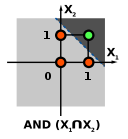
\includegraphics[scale=1]{images/perceptron_and.png}
    \caption{Separacion lineal de la funcion AND.}
  \end{minipage}
\hfill
\begin{minipage}[b]{0.4\textwidth}
    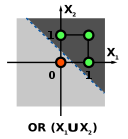
\includegraphics[scale=1]{images/perceptron_or.png}
  \caption{Separacion lineal de la funcion OR.}
  \end{minipage}
\end{figure}
\\Sin embargo, la función XOR no puede ser aprendida por un unico perceptrón, ya que requerie el uso de al menos del lineas para separar las clases. Si se quiere alcanzar esta funcionalidad, es necesario utilizarse al menos una capa mas. Aquí es donde entra en juego el perceptrón multicapa.

\section {Perceptron multicapa}
El perceptrón muticapa tuvo su origen en los años 80, con la idea de solucionar el mayor problema del perceptron simple: no ser capaz de aprender funciones no linealmente separables (como es el caso de la función XOR). Se ha demostrado que es un aproximador universal de funciones.
\\El perceptrón multicapa es un modelo de red neuronal con alimentacion hacia delante, es decir, con conexiones sin bucles (tipo de red feedforward). Está compuesto de varias capas ocultas entre la entrada y la salida de la misma, y caracterizado por tener salidas disjuntas pero relacionadas entre si, ya que la salida de una neurona es la entrada de la siguiente.
\begin{figure}[htp]
\centering
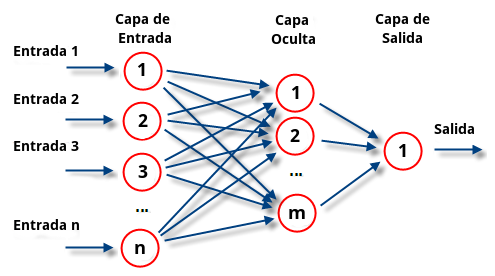
\includegraphics[scale=1.2]{images/multilayerperceptron.png}
\caption{Perceptrón multicapa.}
\end{figure}
\\Las capacidades de decisión de un perceptron multicapa de 2 y 3 capas con una unica neurona de salida se muestran en la siguiente tabla:
\begin{figure}[htp]
\centering
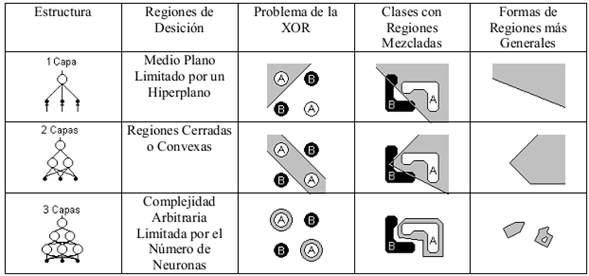
\includegraphics[scale=0.7]{images/perceptron23capas.png}
\end{figure}
\\En el perceptrón multicapa, al igual que en el perceptrón simple, podemos diferenciar una fase de propagación de los valores de entrada hacia delante, y una fase de aprendizaje en la que los datos obtenidos a la salida del perceptrón se van propagando hacia atrás para observar el error y actualizar los pesos de las neuronas. Este algorirmo se llama backpropagation o retropropagación.
\subsection{Propagación}
Imaginemos un perceptrón multicapa con C capas. Llamemos ${W^{C} = W^{c}_{ij}}$ a la matriz de pesos de la capa c y c+1, donde ${W^{c}_{ij}}$ representa el peso de la neurona i de la capa c a la neurona j de la capa c+1. Denominaremos ${U^{C} = u^{c}_{i}}$ al vector de umbrales de las neuronas de la capa c. Se denomina ${a^{c}_{i}}$ a la activación o entrada de la neurona i de la capa c. Las activaciones de las neuronas se calculan de forma distinta dependiendo de la capa en la que nos encontremos.
\begin{itemize}
\item Capa de entrada: la activación se corresponde con el patrón de entrada del perceptrón.
\item Capa oculta: la activación procede de las salidas de las capas anteriores conectadas a las neuronas de esta capa. Esta activación se calcula como la suma de los productos de las activaciones que reciben las neuronas de las capas anteriores multiplicadas por su peso, añadiendoles el umbral, es decir:\\
\begin{equation}
a_{i}^{c} = f(\sum_{j=1}^{n_{c-1}}w_{ji}^{c-1}a_{j}^{c-1}+u_{i}^{c})
\end{equation}
\item Capa de salida: ocurre lo mismo que en las capas ocultas, salvo que ahora la salida de las neuronas se corresponde con la salida de la red.
\end{itemize}
La funcion f es a lo que llamamos funcion de activación. Las funciones de activación mas utilizadas en el perceptrón multicapa son la función sigmoidal y la función tangente hiperbólica. Ambas poseen un intervalo continuo dentro de [0,1] y [-1,1] y vienen dadas por las siguientes ecuaciones.
\begin{itemize}
\item Función sigmoidal ${f_{sigm}(x)=\frac{1}{1+e^{-x}}}$
\item Función tangente hiperbólica ${f_{thip}(x)=\frac{1-e^{-x}}{1+e^{-x}}}$
\end{itemize}
\begin{figure}[htp]
\centering
\vspace{-1.5em}
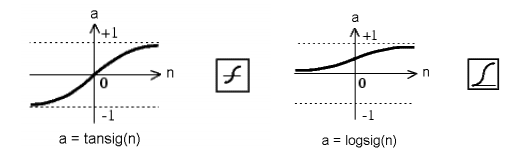
\includegraphics[scale=0.6]{images/tansig_vs_logsig.png}
\end{figure}
Ambas funciones estan relacionadas mediante la expresión ${f_{thip}(x)=2f_{sigm}(x)-1}$, por lo que la utilización de una u otra depende de cual sea mas compatible con el tipo de patrón que se va a utilizar. La funcion sigmoidal tiene un nivel de saturación inferior igual a 0, y la tangente hiperbólica lo tiene a -1.\\
Normalmente, la función de activacion suele ser la misma para todas las neuronas de la red exceptuando las neuronas de la capa de salida, que suelen utilizar dos funciones distintas: la funcion identidad, y la función escalon.
\subsection{Consideraciones de diseño}
A la hora de diseñar un perceptrón multicapa para abordar un problema, el primer paso es determinar la arquitectura de la red. Esto implica determinar tres variables, ya explicadas anteriormente:
\begin{itemize}
\item Función de activación: se elige según el recorrido deseado, pero no influye en la capacidad de la red para resolver el problema.
\item Numero de neuronas de entrada y de salida: viene dado por la definicion del problema. En ocasiones esta afirmación no tiene porque ser del todo cierta, y se ha de proceder a hacer un analisis previo basandose en tecnicas de analisis de correlacion, de sensebilidad, de importancia relativa...
\item Numero de capas ocultas: pese a ser una variable que ha de definir el diseñador, no existe un mé'todo que determine el numero óptimo de neuronas ocultas para resolver el problema. Partiendo de una arquitectura ya entrenada, se van realizando pequeños cambios en el numero de neuronas/capas ocultas para buscar así el diseño optimo, ya que existen muchos tipos de arquitectura capaces de resolver un mismo problema.
\end{itemize}
\subsection{Algoritmo de Retropropagacion o Backpropagation}
Como se ha comentado anteriormente, el proceso de aprendizaje del perceptron multicapa consiste en propagar hacia atrás cierta informacion desde la salida del perceptrón hasta su entrada. Esta información será el error entre la salida obtenida y la salida esperada, con el objetivo de que en las siguientes iteraciones la salida obtenida se aproxime lo máximo prosible a la salida esperada. Por tanto, nos encontramos ante un algoritmo de aprendizaje supervisado.\\
Hay muchos errores que se pueden utilizar, pero el perceptrón multicapa usa la función error cuadrático medio, que se define como:
\begin{equation}
e(n) = \frac{1}{2}\sum_{i=1}^{n_{c}}(s_{i}(n)-y_{i}(n))^{2}
\end{equation}
siendo n cada una de las iteraciones del aprendizaje. El error obtenido e(n) es el error de una sola iteracion, por lo que si queremos entrenar la red con varios patrones, el error medio de esta será ${E=\frac{1}{N}\sum_{n=1}^{N}e(n)}$. En resumen, el perceptrón multicapa aprende encontrando el minimo de la función de error.\\
Aunque el aprendizaje debe llevarse a cabo minimizando el error total, los metodos más utilizados son los basados en metodos de gradiente estocástico, que consisten en minimizar el error en cada patron e(n). Por tanto, aplicando el metodo de gradiente descendiente, cada peso de la red w se actualiza para cada patrón de entrada n, y siendo ${\alpha}$ la tasa de aprendizaje, de acuerdo con la siguiente ecuacion:
\begin{equation}
w(n)=w(n-1)-\alpha \frac{\partial e(n)}{\partial w}
\end{equation}
Dado que las neuronas de la red están agrupadas en capas ocultas segun niveles, es posible aplicar el metodo del gradiente descendente de forma eficiente en todas las neuronas, llevando a cabo el algoritmo de retropropagacion o regla delta generalizada.

\subsection{Regla delta generalizada}
Como ya se ha comentado, la regla delta generalizada no es mas que una forma eficiente de aplicar el método de gradiente a los parametros de la arquitectura (pesos y umbrales). Su aprendizaje es supervisado. Su uso consiste en ajustar pesos y bias tratando de minimizar la suma del error cuadrático. Para ello, se cambian dichas variables en la dirección contraria a la pendiente del error.\\
Las redes neuronales entrenadas mediante esta técnica, dan respuestas mas que razonables cuando al sistema se le presentan entradas que nunca habia analizado. A una nueva entrada, le hará corresponder una entrada similar a la salida obtenida para un patrón de entrenamiento, siendo éste similar al patrón presentado a la red. Esta es una de las grandes propiedades de la regla delta, su capacidad de generalicación.\\
Podriamos describir su funcionamiento básico en una serie de pasos:
\begin{itemize}
\item Se introduce un vector de entrada, y se calcula su salida.
\item Se calcula el error
\item Se determina en que direccion se deben cambiar los pesos para minimizar el error
\item Se determina la cantidad en la que se cambiará cada peso
\item Se modifican los pesos.
\item Se repiten los pasos del 1 al 5 con todos los patrones de entrenamiento, hasta que el error de los vectores sea lo más reducido posible.
\end{itemize}

\subsection{Tasa de aprendizaje}
La tasa de aprendizaje (${\alpha}$) es un parámetro que determina la velocidad a la que van a cambiar los pesos de las conexiones de la red. Tiene un rango [0,1], siendo los valores mas cercanos a cero los que hacen que los pesos cambien poco a poco, acercandose lentamente a la convergencia, y los cercanos a uno los que hacen que la red converja mas rapidamente al principio, pero siendo posible que los pesos oscilen demasiado al encontrar el peso óptimo final. Por esta razón es importante encontrar una tasa de aprendizaje óptima.\\
Aquí es donde entra en juego un segundo termino llamado momento (${\eta}$), que pondera cuanto queremos que influya lo que los pesos han cambiado en la anterior iteración. Con ello, sabremos que si los pesos han cambiado mucho, es que estamos aun lejos del valor de la tasa de aprendizaje óptimo, por lo que avanzaremos en su busqueda mas rapidamente. Por otro lado, si los pesos no han cambiado a penas, sabremos que el valor optimo de ${\alpha}$ está cerca.\\
Podemos modificar la ecuacion 2.XXXXXXXX para añadir esta mejora, de la siguiente manera:
\begin{equation}
w(n) = w(n-1) = - \alpha \frac{\partial e(n)}{\partial w} + \eta \Delta w(n-1)
\end{equation} 
siendo ${\Delta}$w(n-1)=w(n-1)-w(n-2) el incremento que sufrió el parametro w en la anterior iteración.
\subsection{Sobreajuste y early stopping}
El sobreajuste o overfitting es el efecto secundario de sobreentrenar un algoritmo de aprendizaje con ciertos datos para los que ya se conoce el resultado deseado. El algortismo debe alcanzar un estado en el cual sea capaz de predecir otros casos a partir de lo ya aprendido mediante datos de entrenamiento, generalizando para poder resolver distintas situaciones a las ya presentes durante el entrenamiento. No obstante, cuando un sistema se entrena demasiado o se entrena con datos extraños, el algoritmo tiende a quedarse ajustado a unas caracteristicas muy especificas de los datos de entrenamiento, que no representan un estado general de problema. En este estado, nuestro diseño es mas eficaz al responder a muestras del conjunto de entrenamiento, pero ante nuevas entradas el resultado empeora.\\
Una manera de resolver este problema es extraer un conjunto de entradas del dataset de entrenamiento, y utilizarlo de manera auxiliar a modo de validación. Ya que este subconjunto se deja al margen durante el entrenamiento, su objetivo será evaluar el error en la red tras cada epoch, para determinar cuando este empieza a aumentar. Cuando aumente, se prodecerá a detener el entrenamiento y se conservarán los valores de los pesos del ciclo anterior. A este método se le llama early-stopping.

\section{Redes neuronales convolucionales}
Las redes neuronales convolucionales son muy similares a las redes neuronales ordinarias descritas hasta ahora, como el perceptrón multicapa. Las neuronas tienen pesos, sesgos, reciben una entrada con la que realiza un producto escalar y sobre la que aplica una función de activación, tienen una función de perdida...\\
Sin embargo, se utilizan principalmente para resolver el principal problema que tienen las redes neuronales ordinarias: el tratamiento de imagenes. Pese a que con las redes neuronales estandar es posible manejar imagenes como es el caso del dataset MNIST, en cuanto las imagenes aumentan su tamaño y calidad esto se vuelve intratable. Al tratarse de neuronas totalmente conectadas, provocariamos un desperdicio de recursos así como un rapido sobreajuste.\\
Las redes neuronales convolucionales trabajan dividiendo y modelando la información en partes mas pequeñas, y combinando esta información en las capas mas profundas de la red. Por ejemplo, en el caso del tratamiento de una imagen, las primeras capas tratarían de detectar los bordes de las figuras. Las siguientes capas buscarían combinar los patrones de detección de bordes para conseguir formas mas simples, y aplicar patrones de posición de objetos, iluminacion... Por ultimo, en las últimas capas se intentará hacer coincidir la imagen con todos los patrones descubiertos, para conseguir una predicción final de la suma de todos ellos. Así es como las redes neuronales convolucionales consiguen modelar una gran cantidad de datos, diviendo previamente el problema en partes para conseguir predicciones mas sencillas y precisas.
\subsection{Estructura}
En general, todas las redes neuronales convoluciones estan formadas por una estructura compuesta por 3 tipos de capas:
\subsubsection{Capa convolucional}
Esta capa le da nombre de la red. En vez de utilizar la multiplicación de matrices como en la redes neuronales estandar, se aplica un operación llamada convolución. Esta operación recibe como entrada una imagen, y sobre ella aplica un filtro que nos devuelve su mapa de caracteristicas, reduciendo así el tamaño de sus parametros. La convolución utilizada tres ideas que ayudan a mejorar cualquier sistema sobre el que se aplique machine learning:
\begin{itemize}
\item{Iteracciones dispersas:}
Al aplicar un filtro de menos tamaño sobre la entrada, reducimos bastante el numero de parámetros y calculos.
\item{Parametros compartidos:}
Compartir parametros entre los distintos tipos de filtros ayuda a mejorar la eficiencia del sistema.
\item{Representaciones equivariantes:}
Si las entradas cambian, las salidas cambian de forma similar.
\end{itemize}
Además, la convolucion proporciona herramientas para trabajar con entradas de tamaño variable, lo que es muy util para trabajar con imagenes (cada imagen tiene un numero de pixeles distinto). Se basa en un operador matemático que transforma dos funciones f y g, en una tercera, que en cierto sentido, represenrta la magnitud en la que se superponen f y una versión transladada e invertida de g.
\begin{figure}[htp]
\centering
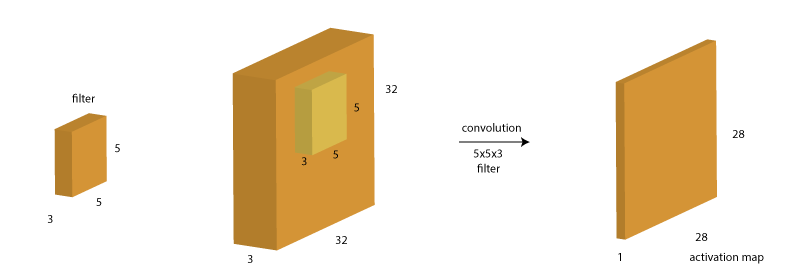
\includegraphics[scale=0.7]{images/conv_layer.png}
\caption{Funcionamiento de capa convolucional}
\end{figure}\\
\subsubsection{Capa de reducción o pooling}
Esta capa se coloca generalmente después de la capa convolucional. Reduce la cantidad de parametros a analizar reduciendo las dimensiones espaciales (ancho x alto), quedandose con las características mas comunes. La operación que lleva a cabo esta capa también se llama reduccion de muestreo, ya que la reducción de tamaño implica tambien una perdida de información. Sin embargo, para un red neuronal, este tipo de perdida puede ser beneficioso debido a:
\begin{itemize}
\item La reducción del tamaño provoca una menor sobrecarga de calculo en las proximas capas de la red.
\item Reducir el sobreajuste
\end{itemize}
La operacion que se suele aplicar en esta capa es "max-pooling", que divide la imagen de entrada en un conjunto de rectángulos y respecto a cada uno de ellos, se queda con el máximo valor.
\begin{figure}[htp]
\centering
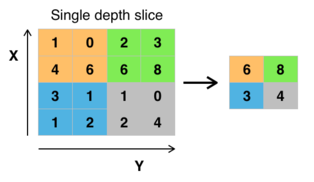
\includegraphics[scale=0.7]{images/max_pooling.png}
\caption{Max-pooling aplicado a una imagen}
\end{figure}
\subsubsection{Capa clasificadora totalmente conectada}
Una vez que la imagen ha pasado por las capas convolucionales y de pooling, las redes convolucionales normalmente usan capas completamente conectadas en las que cada pixel se trata como una neurona independiente, separada como si se tratase de una red neuronal estandar. Esta ultima capa clasificadora tendrá tantas neuronas como el numero de clases a predecir, y nos ofrecerá el resultado final de la red.

\section{Redes neuronales recurrentes}
Los humanos no empiezan a pensar de cero a cada segundo. Por ejemplo, mientras leemos, entendemos cada palabra basandonos en el contexto que forman las palabras anteriores. No desperdiciamos los ideas anteriores, si no que estas tienen persistencia en la memoria.\\
Las redes neuronales tradicionales no cuentan con esta capacidad, y es su mayor defecto. Por ejemplo, imaginemos el caso en el que queremos clasificar que clase de evento está pasando en una punto de una película. No está muy claro como una red neuronal tradicional podría usar razonablemente las escenas anteriores para predecir las siguientes.\\
Y aquí es donde entran en juego las redes neuronales recurrentes, ya que resuelven este problema. Su principal característica es que son redes con bucles, que permiten que la información persista.\\
\begin{figure}[htp]
\centering
\vspace{-1.5em}
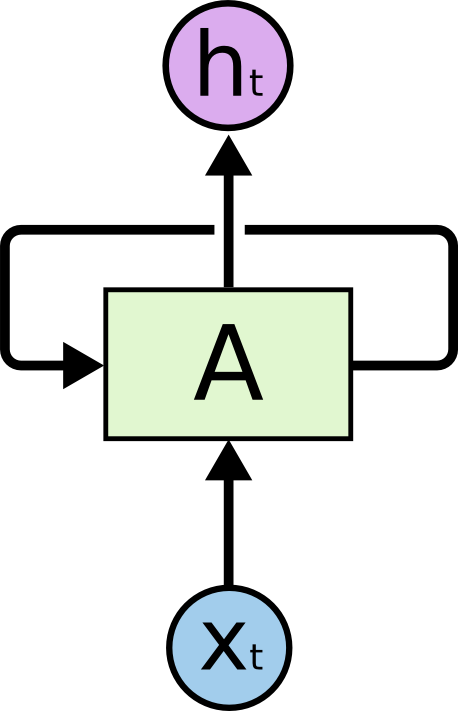
\includegraphics[scale=0.3]{images/rnnrolled.png}
\caption{Ejemplo básico de red neuronal recurrente.}
\end{figure}
\\En el diagrama superior, podemos ver como una parte de la red neuronal, A, recibe una entrada x y devuelve una salida h. El bucle permite que la información pase de un paso de la red al siguiente. Pese a que el concepto de bucle parezca algo extraño, las redes neuronales que cuentan con ellos no son tan distantes de la redes neuronales tradicionales. Una red neuronal recurrente puede ser creada utilizando multiples copias de la misma red, pasando el mensaje o salida al nodo sucesor. Si desenrollamos el bucle, tendriamos algo parecido a lo siguiente:\\
\begin{figure}[htp]
\centering
\vspace{-1.5em}
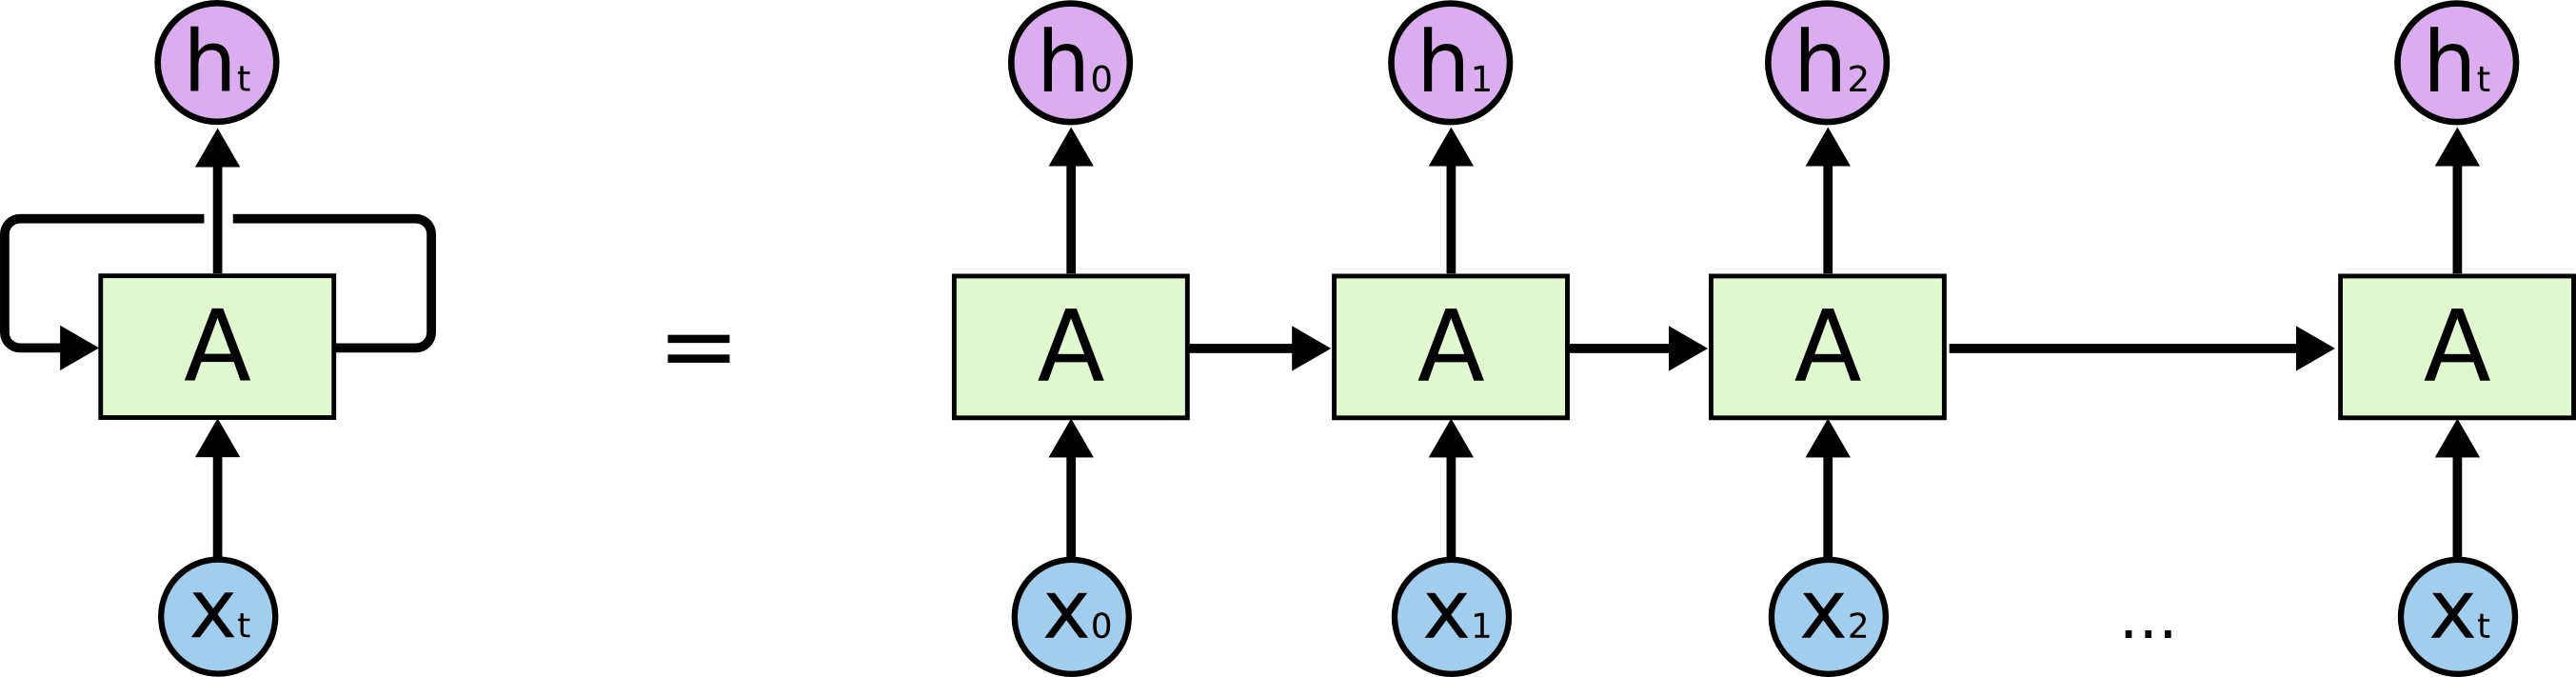
\includegraphics[scale=0.3]{images/RNNunrolled.png}
\caption{Red neuronal recurrente desenrollada.}
\end{figure}
\\Esta forma de cadena hace preveer que las redes neuronales recurrentes estan intimamente recolacionas con secuencias y listas. En los ultimos años, se han logrado autenticos grandes éxitos aplicando las RNN para resolver problemas: reconocimiento de discursos, modelación de lenguajes, traducciones, captación de imagenes... Un factor clave en estos exitos es la uso de LSTMs, un tipo muy especial de redes neuronales recurrentes, que trabajan por muchas razones de forma mas eficiente que la version estándar.
\subsubsection{El problema de la longitud de las dependencias.}
Uno de los intereses de las RNNs es la idea de conectar información antigua con la tarea actual. En temas de video, sería util por ejemplo utilizar frames anteriores para entender el actual, pero... ¿puedes las RNN hacer esto? Depende.\\
Algunas veces, solo necesitamos utilizar información reciente para la tarea actual. Por ejemplo, en temas de modelación de lenguaje, para adivinar la siguiente palabra en un contexto, en la mayoría de los casos bastaría con analizar la frase en la que se encuentra. Sin embargo, hay casos en los que necesitamos acceder a un contexto mas grande. Desafortunadamente, a medida que el espacio entre la informacion requerida y la tarea actual aumental, las RNN cada vez tardan mas en aprender a conectar la información.\\
\begin{figure}[htp]
\centering
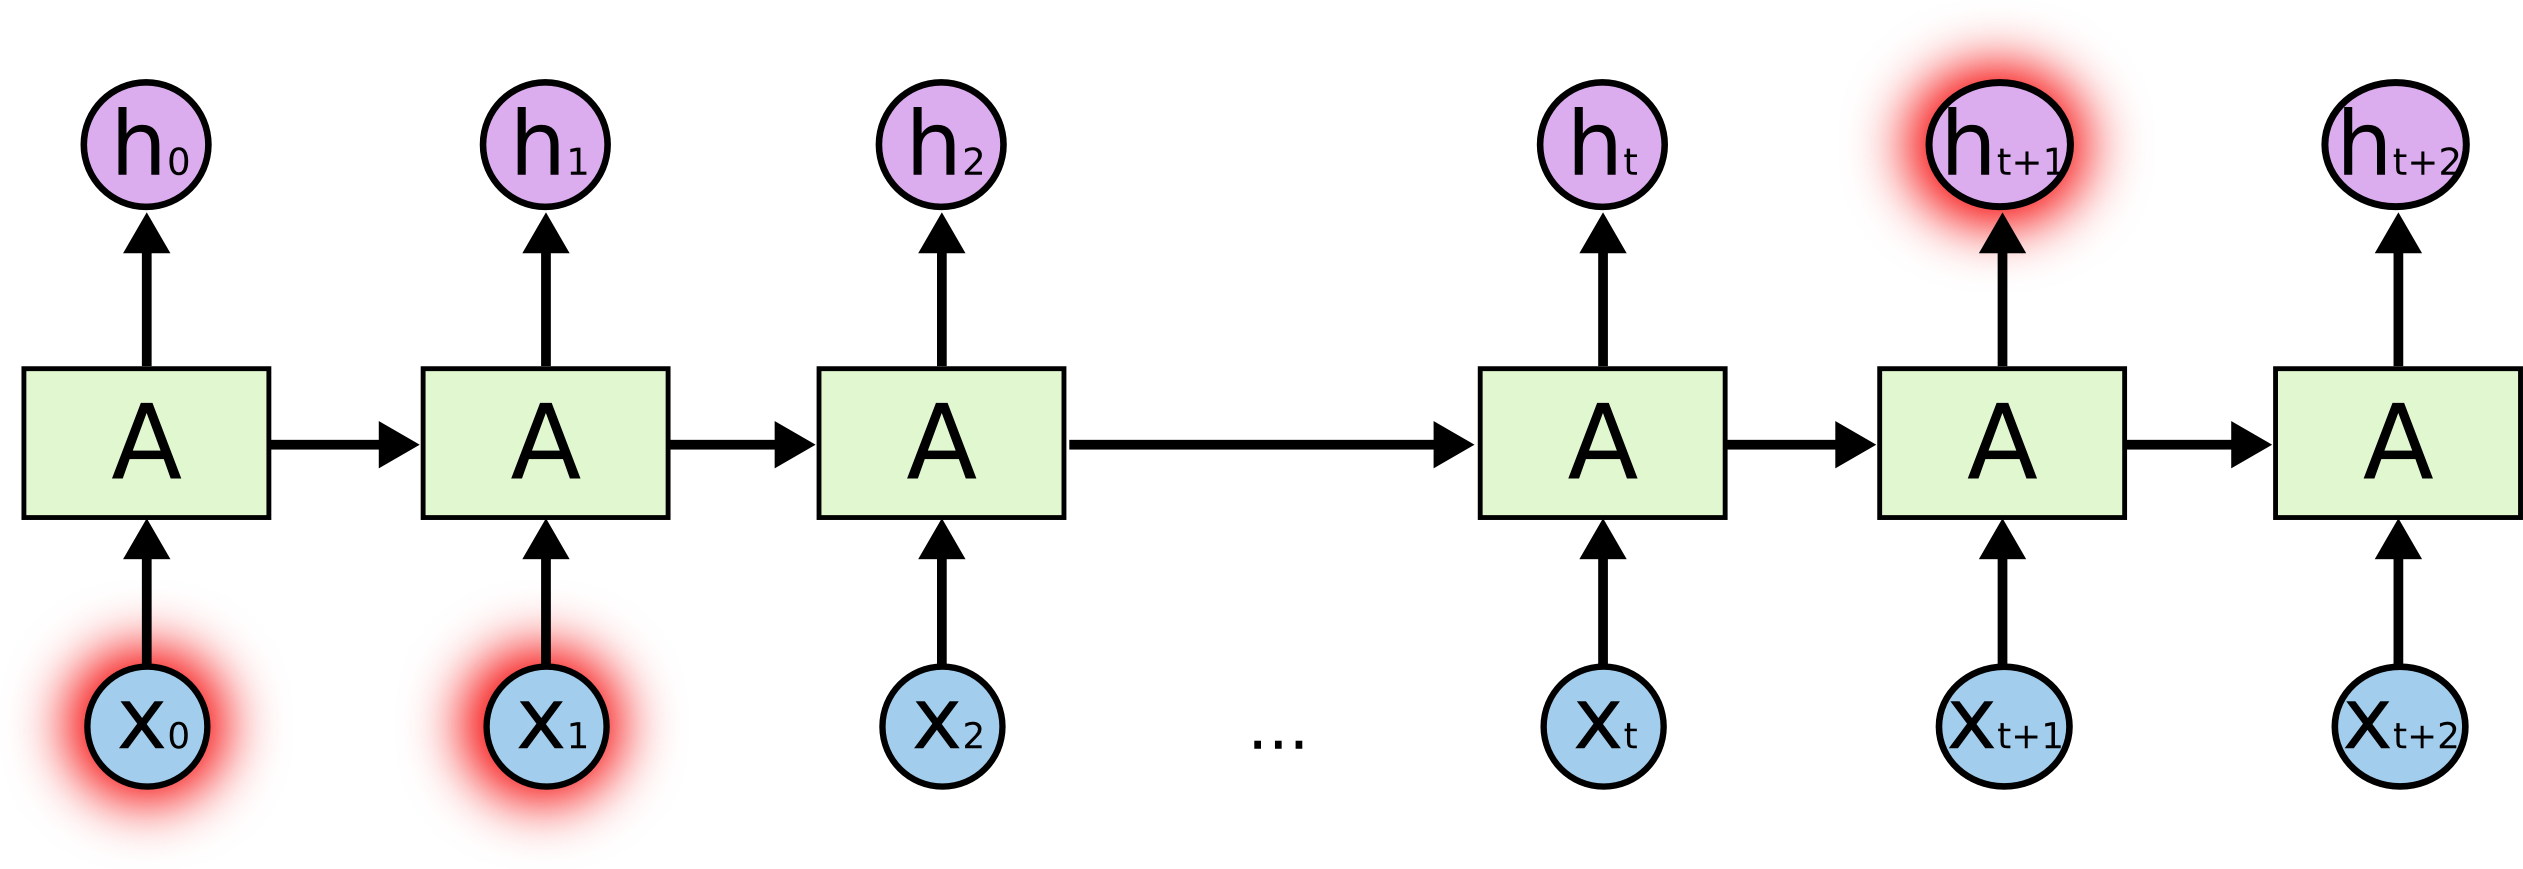
\includegraphics[scale=0.3]{images/RNN-longtermdependencies.png}
\caption{Red neuronal recurrente desenrollada.}
\end{figure}
\\En teoria, las RNN son perfectamente capaces de resolver este problema (long-term dependencies), pero en la práctica no lo parece tanto. En 1991, Hochreiter estudió este problema, y encontró algunas razones por las que las RNN encuentran dificultades a la hora de aprender información sobre grandes contextos. Por suerte, las redes LSTMs solventan estos problemas.
\subsection{Redes LSTM}
Las redes Long Short Term Memory (normalmente llamadas LSTMs) son un tipo especial de redes neuronales recurrentes descritas por primera vez en 1997 por Hochreiter \& Schmidhuber, capaces de aprender una larga lista de dependencias en largos periodos de tiempo.\\
Todas las redes neuronales recurrentes tienen forma de cadena al repetir sus modulos. En las RNN estandar, el modulo repetidor tiene una estructura muy simple, con una sola capa, como podria ser la de tipo tanh. Las redes LSTM tambien tienen forma de cadena, pero el modulo repetidor en vez de tener una sola capa, tiene cuatro.
\begin{figure}[htp]
\centering
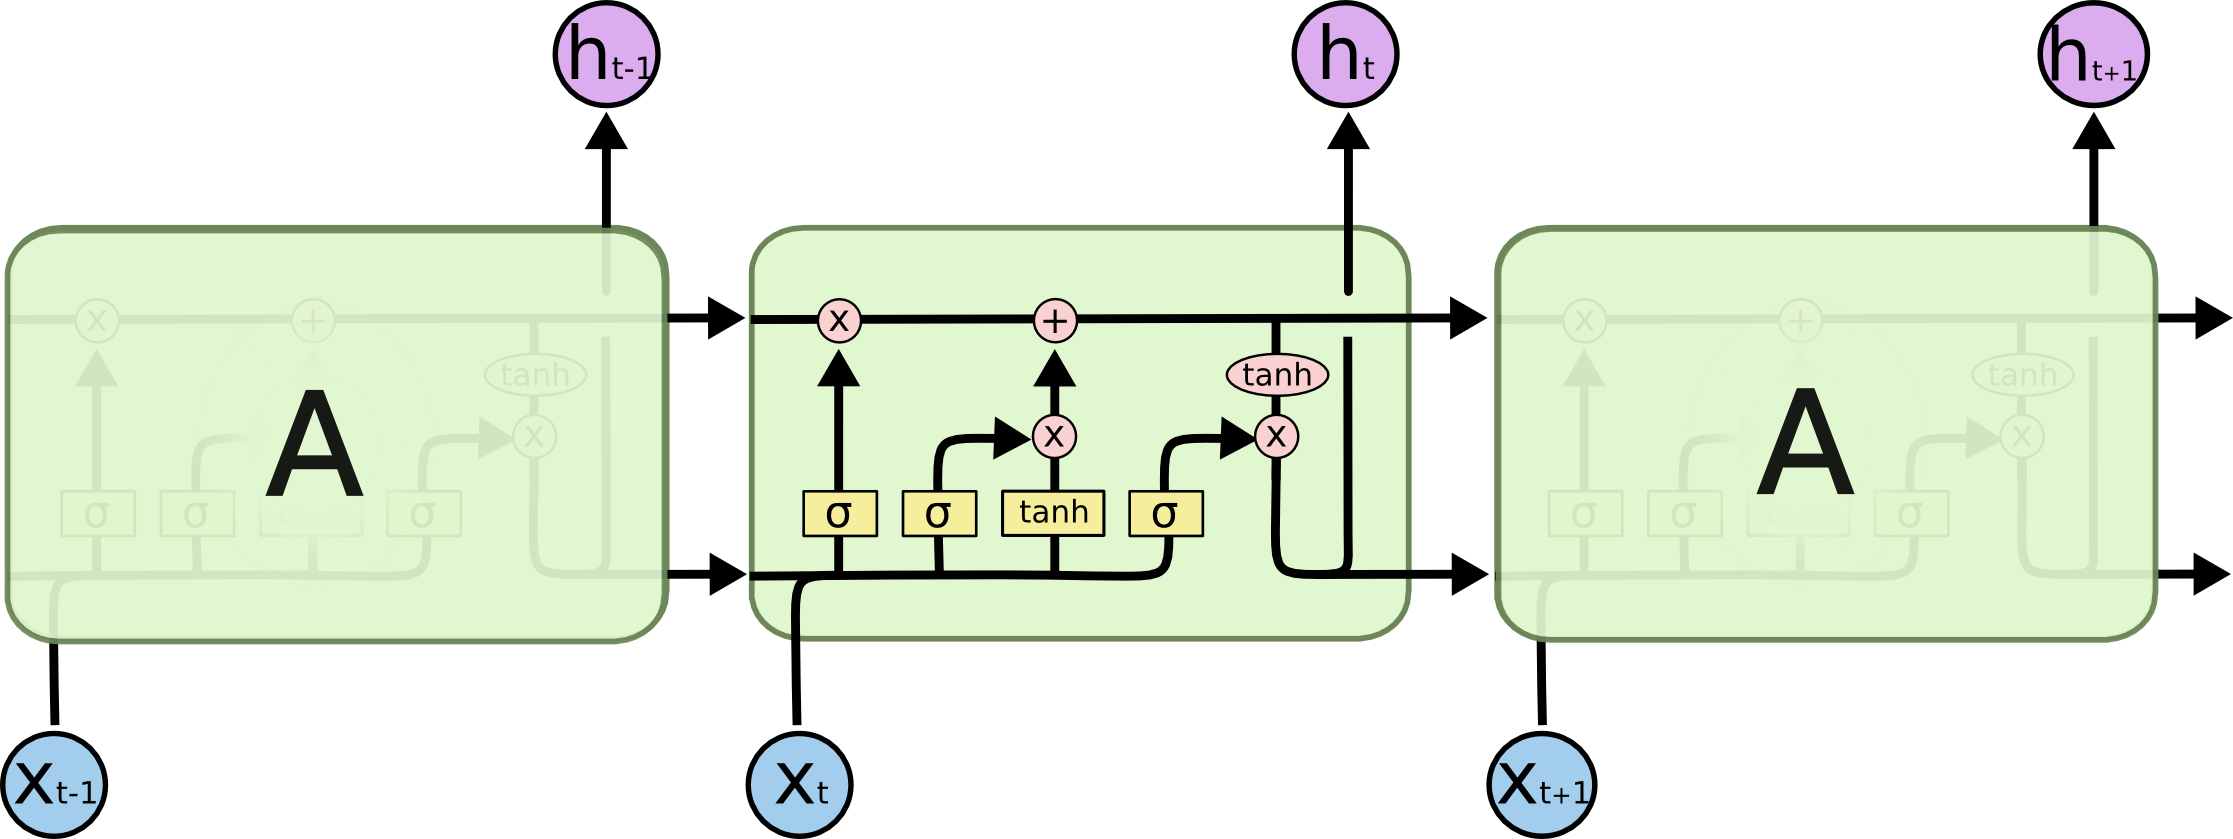
\includegraphics[scale=0.35]{images/LSTM3-chain.png}
\caption{Estructura del modulo repetidor.}
\end{figure}
\begin{figure}[htp]
\centering
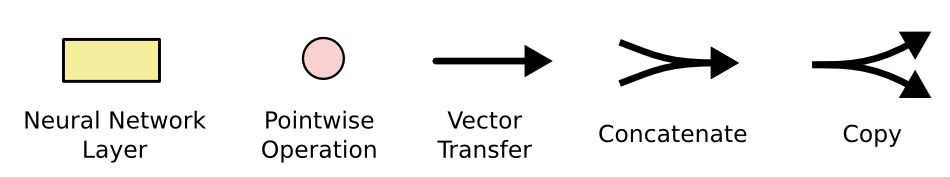
\includegraphics[scale=0.2]{images/LSTM2-notation.png}
\caption{Notación del modulo repetidor.}
\end{figure}
\\La clave de las redes LSTMs se encuentra en el estado de la celda, es decir, en la linea horizontal de la parte superior del diagrama, ya que recorre toda la cadena con solo algunas pequeñas interacciones. Para la información, es muy facil recorrer la red sin ser alterada.\\
La red tambien tiene la habilidad de borrar o añadir información al estado de la celda, reguladas cuidadosamente por estructuras llamadas puertas. Estas puertas son una manera de permitir opcionalmente a la información circular o no. Están compuestas por un capa sigmoide y una operación de multiplicación. La salida de la capa sigmoide alterna entre 0 y 1, describiendo si la informacion fluye o no. Una red LSTM tiene 3 de estas puertas, para proteger y controlar el estado de la celda.\\\\
Las redes neuronales LSTM siguen una serie de pasos para decidir que información se va a ir almacenando o borrando. Podemos destacar los siguientes:
\begin{enumerate}
\item \textbf{Decidir que información despreciar}. Esta decisión la toma la capa sigmoide, que  devuelve una salida igual a 1 si se busca mantener la informacion, o 0 si queremos deshacernos de ella.\\
Volvamos al ejemplo de modelación del lenguaje, donde se quiere predecir una palabra basandose en las anteriores. En este problema, el estado de la celda almacenará el genero del sujeto, para usar los pronombres adecuados. Cuando nos encontremos un nuevo sujeto, olvidaremos el genero del anterior ya que no será de utilidad.
\item \textbf{Decidir que información se va a almacenar}. Consta de dos partes: primero, una capa sigmoide deciden que valores son actualizados. Después, una capa tanh crea un vector con los nuevos valores candidatos, que pueden ser añadidos al estado.\\
En el ejemplo anterior, se decidiría que queremos añadir el genero del nuevo sujeto al estado de la celda, para reemplazar el viejo que queremos olvidar.
\item \textbf{Actualizar el estado de la celda}. En el paso anterior se decide que hacer, y ahora toca hacerlo. Multiplicamos el viejo estado por la salida de la capa sigmoide del primer paso, olvidando las cosas que decidimos olvidar. A esto, le sumamos el producto de la salida de la capa sigmoide y de la capa tanh del segundo paso. Con ello, conseguimos saber los nuevos valores candidatos, escalados segun la decisión de actualizar el estado de la celda.\\
En el caso de modelado de lenguaje, ahora es cuando desechamos la informacion sobre el genero del viejo sujeto, y añadimos la nueva informacion, como decidimos en los pasos anteriores.
\item \textbf{Decidir la salida basandonos en el estado de la celda, pero de manera filtrada}. Primero, mediante una capa sigmoide, se decide que partes del nuevo estado de la celda se van a sacar como salida. Después, se pasa el estado de la celda por una capa tanh para tener valores entre -1 y 1, y lo multiplicamos por la salida de la capa sigmoide, para sacar solo las partes que decidamos.\\
En el ejemplo de modelado de lenguaje, una vez que nos encontremos con el nuevo sujeto, sacaremos informacion a cerca de él como puede ser el si es singular o plural, para después poder conjugar correctamente el verbo que le sigue.
\end{enumerate}
Como he comentado anteriormente, la mayoría de los mejores resultados utilizando redes recurrentes, es mediante las redes LSTMs. Pero a pesar de que su descubrimiento ha sido un gran hito, todavia quedan metas por cumplir. Uno de ellos sería dotar a las RNN de una capacidad para decidir que información consultar en una fuente muy grande de información. Por ejemplo, si estamos usando redes RNN para crear un titulo que describa una imagen, sería util elegir que partes de la imagen usar para cada palabra.
\label{ch:teoria} 
\chapter{Keras}
\section{Introducción}
Keras es una librería de redes neuronales escrita en Python y capaz de correr tanto en Tensorflow como en Theano. Sus principales características son:
\begin{itemize}[noitemsep]
\item Fácil y rápido prototipado gracias a su modularidad, minimalismo y extensibilidad.
\item Soporta tanto redes neuronales convolucionales como recurrentes (así como la combinación de ambas)
\item Soporta esquemas de conectividad arbitrarios (incluyendo entrenamiento multi-entrada y multi-salida)
\item Corre en CPU y GPU
\item Es compatible con Python 2.7-3.5
 \end{itemize}

 \section{Instalación}
 Para la instalacion de Keras, son necesarias las siguientes dependencias:
 \begin{itemize}[noitemsep]
\item numpy y scipy
\item pyyaml
\item HDF5 y h5py (Opcional, pero requírido si se usan funciones para cargar/guardar modelos)
\item cuDNN (Opcional pero recomendado si se usan CNNs)
\item Tensorflow o Theano
 \end{itemize}
Existen 2 modos de instalacion:
 \begin{itemize}[noitemsep]
 \item Desde PyPI: \lstinline{sudo pip install keras}
 \item Desde repositorio Keras (https://github.com/fchollet/keras/tree/master/keras): \lstinline{sudo python setup.py install}
 \end{itemize}
 Por defecto, Keras usa Tensorflow como motor backend. Sin embargo, esta opción puede ser configurada. La primera vez se ejecuta Keras, se crea un fichero de configuración en "/.keras/keras.json", que puede ser modificado.
\begin{lstlisting}
    "image_dim_ordering": "tf",
    "epsilon": 1e-07,
    "floatx": "float32",
    "backend": "tensorflow"
\end{lstlisting}

\section{Modelos}
Hay 2 tipos de modelos disponibles para su implementacion en Keras: el modelo secuencial, y la clase Model (más general). Ambos modelos presentan varias funciones en común, como \lstinline{summary()}, \lstinline{get_config()} o \lstinline{to_json()} que devuelven información basica sobre el modelo, o \lstinline{get\_weights()} y \lstinline{set\_weights()}, las funciones getter y setter para los pesos del modelo.
\subsection{Modelo secuencial}
Las funciones básicas del modelo secuencial son:
\begin{itemize}
\item \lstinline{compile(self, optimizer, loss, metrics=[], sample_weight_mode=None)} : Configura el proceso de aprendizaje.
\item \lstinline{fit(self, x, y, batch_size=32, nb_epoch=10, verbose=1, callbacks=[], validation_split=0.0, validation_data=None, shuffle=True, class_weight=None, sample_weight=None)} : Entrena el modelo para un número fijado de ciclos.
\item \lstinline{evaluate(self, x, y, batch_size=32, verbose=1, sample_weight=None)} : Calcula la función de perdida dados unos datos de entrada, lote por lote.
\item \lstinline{predict(self, x, batch_size=32, verbose=0)} : Genera predicciones para unos valores de entrada.
\end{itemize}
\subsection{Clase Model de la API}
Con la clase Model, dadas una entrada y una salida, podemos inicializar nuestro modelo de la siguiente forma:
\begin{lstlisting}[language=Python]
a = Input(shape=(32,))
b = Dense(32)(a)
model = Model(input=a, output=b)
\end{lstlisting}
En caso de que tengamos múltiples conjuntos de entradas y de salidas, también podríamos inicializarlo de la siguiente manera:
\begin{lstlisting}[language=Python]
model = Model(input=[a1, a2], output=[b1, b3, b3])
\end{lstlisting}
\section{Capas}
\subsection{Funciones básicas de las capas}
A la hora de diseñar las capas de nuestra red neuronal, tenemos una serie de funciones disponibles:
\begin{itemize}
\item Dense: Para capas regulares totalmente conectadas.\\
\lstinline{keras.layers.core.Dense(output_dim, init='glorot_uniform', activation='linear', weights=None, W_regularizer=None, b_regularizer=None, activity_regularizer=None, W_constraint=None, b_constraint=None, bias=True, input_dim=None)}\\
Ejemplo de uso: \lstinline{model.add(Dense(32, input_dim=16))} sería un modelo que contaría con una array de entrada de tamaño 16, y de salida de 32.
\item Activation: Se aplica una función de activación a una salida. Las principales funciones que nos ofrece Keras son:
\begin{itemize}
\item softmax: generalización de la función logística.
\item softplus
\item softsign
\item relu: función rectificadora
\item tanh: función tangente hiperbólica
\item sigmoid: función sigmoide
\item hard\_sigmoid
\item linear: función lineal
\end{itemize}
Podemos encontrar funciones de activación mas avanzadas como PReLu o LeakyReLU en el modulo \lstinline{keras.layers.advanced_activations}.\\
Ejemplo de uso: \lstinline{model.add(Activation('tanh'))}
\item Dropout: Proporciona una manera simple de prevenir que se produzca sobreajuste.\\
\lstinline{keras.layers.core.Dropout(p)}
\item Reshape: Transforma la salida en una forma concreta.\\
Ejemplo de uso: \lstinline{model.add(Reshape((3, 4), input_shape=(12,)))} definiría una capa de salida de 3x4 para nuestro modelo.
\item Permute: Transforma la dimensión de la entrada en un patrón definido.\\
Ejemplo de uso: \lstinline{model.add(Permute((2, 1), input_shape=(10, 64)))}
\end{itemize}

\subsection{Capas convolucionales}
Keras presenta diversas funciones para desarrollar capas convolucionales según las dimensiones de su entrada. La mas destacable, a modo de ejemplo, podría ser:\\
\lstinline{Convolution2D(nb_filter, nb_row, nb_col, init='glorot_uniform', activation=None, weights=None, border_mode='valid', subsample=(1, 1), dim_ordering='default', W_regularizer=None, b_regularizer=None, activity_regularizer=None, W_constraint=None, b_constraint=None, bias=True)}\\\\
Además de la versión en 2D, Keras nos ofrece funciones para entradas de 1 dimensión o 3 dimensiones. A parte, tenemos funcionalidades para desarrollar capas convolucionales dilatadas (AtrousConvolution2D), hacer deconvolución (Deconvolution2D), cropping (Cropping2D)...
\subsection{Capas pooling}
Al igual que ocurre con las capas convolucionales, Keras ofrece un buen numero de funciones para desarrollar capas pooling en redes convolucionales, dependiendo de las dimensiones de la entrada. Como en el caso anterior, una función representativa sería:\\
\lstinline{MaxPooling2D(pool_size=(2, 2), strides=None, border_mode='valid', dim_ordering='default')}\\\\
Si en vez de utilizar la función máximo se requiere que nuestra capa utilice otro tipo de algoritmos, Keras también nos ofrece funciones como: AveragePooling2D, GlobalMaxPooling2D, GlobalAveragePooling2D... Además de sus variantes para 1D y 3D.
\subsection{Capas recurrentes}
Keras presenta 3 tipos de capas recurrentes:
\begin{itemize}[noitemsep]
\item SimpleRNN : Red recurrente totalmente conectada cuya salida realimenta la entrada.
\item LSTM : Long-Short Term Memory unit
\item GRU : Gated Recurrent Unit
\end{itemize}

\section{Preprocesado}
Keras cuenta con una serie de funciones para procesar tanto modelos secuenciales, como texto, como imágenes. Las más importantes son:
\begin{itemize}
\item Modelos secuenciales: \lstinline{pad_sequences(...)} transforma una lista en un array 2D.
\item Texto: \lstinline{text_to_word_sequence(...)} separa una frase en palabras, \lstinline{one_hot(...)} codifica un texto en una lista de palabras indexadas en un vocabulario de tamaño n...
\item Imágenes: \lstinline{ImageDataGenerator(...)} genera ciclos con los datos de la imagen con aumento en tiempo real.
\end{itemize}
\section{Funciones de pérdida}
La función de perdida es uno de los dos parámetros necesarios para compilar un modelo. Algunas de las funciones mas conocidas que nos proporciona Keras son:
\begin{itemize}[noitemsep]
\item \lstinline{mean_squared_error(y_true, y_pred)} : Calcula el error cuadrático medio.
\item \lstinline{mean_absolute_error / mae} : Calcula el error medio absoluto.
\item \lstinline{binary_crossentropy}: Calcula la entropía cruzada en problemas de clasificación binaria. También conocida como perdida logarítmica.
\end{itemize}
\section{Optimizadores}
El optimizador es otro de los dos valores necesarios para compilar un modelo (junto con la función de pérdida). En los ejemplos que se describirán mas adelante, se usará el optimizador Adam.
\begin{itemize}
\item \lstinline{Adam(lr=0.001, beta_1=0.9, beta_2=0.999, epsilon=1e-08, decay=0.0)}
\end{itemize}
Adam es un algoritmo para la optimización basado en el gradiente de primer orden de funciones estocásticas objetivas. Está basado en estimaciones adaptativas de momentos de orden inferior. Este método es sencillo de implementar, es eficiente computacionalmente hablando, necesita poca capacidad de memoria, y es muy bueno en problemas con una gran cantidad de datos y/o parámetros.
\section{Activadores}
El modo de activación puede ser implementado mediante una capa Activation (\lstinline{model.add(Dense(64)); model.add(Activation('tanh')))}, o mediante un parámetro que soportan todas las capas (\lstinline{model.add(Dense(64, activation='tanh'))}).\\
Las funciones más comunes son:
\begin{itemize}[noitemsep]
\item softmax
\item softsign
\item tanh
\item sigmoid
\item linear
\end{itemize}
\section{Callbacks}
Los callbacks son una serie de funciones que pueden ser aplicadas en ciertos momentos del proceso de entrenamiento. Estos callbacks pueden ser utilizados para echar un vistazo a los estados internos así como a las estadísticas del modelo que estamos entrenando. Para utilizarlos, basta con pasar como argumento a la función \lstinline{fit(...)} una lista de métodos, que serán llamados en cada fase del entrenamiento.\\
Las principales funciones son:
\begin{itemize}
\item \lstinline{BaseLogger()}: Se aplica en todo modelo de Keras, y acumula la media de las métricas por ciclo.
\item \lstinline{Callback()}: Clase base abstracta, utilizada para crear nuevos callbacks. Como parámetros, recibe los propios para configurar el entrenamiento (numero de ciclos, verbosidad...), así como la instancia del modelo que queremos entrenar.
\item \lstinline{ProgbarLogger()}: Callback que pinta métricas en la salida estándar (stdout).
\item \lstinline{History()}: Callback aplicado en cada modelo Keras, que almacena eventos en un objeto de tipo History.
\item \lstinline{ModelCheckpoint(...)}: Almacena el modelo después de cada ciclo. Como argumentos recibe el fichero donde dejar la información, la cantidad de de elementos a monitorizar, el modo de verbosidad, un booleano para decidir si sobreescribir o no el mejor modelo, el modo, y otro booleano para guardar solo pesos o información de todo el modelo.
\end{itemize}
\section{Datasets}
Keras cuenta con una serie de dataset ya predefinidos y listos para realizar nuestras pruebas:
\begin{itemize}
\item \textbf{CIFAR10}: dataset que cuenta con 50.000 imágenes a color de entrenamiento, a clasificar en 10 categorías, y 10.000 imágenes para testear los resultados. También existe una versión con 100 categorías (\textbf{CIFAR100}).
\item \textbf{Clasificación de sentimientos en reviews de IMDB}: Este dataset cuenta con 25.000 películas etiquetadas según el sentimiento (bueno/malo). Estas reviews han sido preprocesadas, y las palabras han sido indexadas según su frecuencia.
\item \textbf{MNIST}: dataset que contiene 60.000 imágenes en blanco y negro de 10 tipos de dígitos, y 10.000 imágenes para testear los modelos.
\end{itemize}
\section{Inicializadores}
Los inicializadores definen la manera de inicializar los pesos de las capas de nuestro modelo. El argumento usado en para definir este inicializador en las capas es \textbf{init}. Las opciones mas comunes son:
\begin{itemize}[noitemsep]
\item uniform
\item normal
\item identity
\item zero
\end{itemize}
\section{Regularizadores}
Los regularizadores permiten aplicar penalizaciones en las capas durante la optimización. Estas penalizaciones se incorporan a la función de perdida que la red optimiza.\\
Ejemplo de uso:
\lstinline{model.add(Dense(64, input_dim=64, W_regularizer=l2(0.01), activity_regularizer=activity_l2(0.01)))}
\section{Visualización}
El módulo \textbf{keras.utils.visualize\_util} proporciona funciones útiles para pintar gráficamente un modelo (acompañado del uso de graphviz). La siguiente función pintaría una gráfica del modelo y lo guardaría en un fichero .png.\\
\lstinline{plot(model, to_file='model.png')}
\section{Wrapper para Scikit-Learn API}
Keras presenta compatibilidad con Scikit-Learn API. Se pueden usar modelos Keras secuenciales como parte del ciclo de trabajo de Scikit-Learn mediante sus wrappers. Hay 2 disponibles:
\begin{itemize}[noitemsep]
\item \lstinline{KerasClassifier(build_fn=None, **sk_params)} : Implementa una interfaz de clasificación.
\item \lstinline{KerasRegressor(build_fn=None, **sk_params)} : Implementa una interfaz de regresión.
\end{itemize}
El primer argumento es la instancia de la clase o la función a llamar, y el segundo los parámetros del modelo y de ajuste.

\chapter{Ejemplos de uso de Keras}
\lsection{Problema de diabetes - Regresión logística}
Como primer ejemplo, se va a utilizar el dataset de diabetes en los indios americanos. Este conocido dataset se puede adquirir en el repositorio de UCI Machine Learning, y describe información médica de pacientes indios, así como si han tenido diabetes en los siguientes 5 años.\\
La información médica especificada es la siguiente:
\begin{itemize}[noitemsep]
\item Número de embarazos.
\item Concentración de glucosa.
\item Presión en sangre.
\item Tamaño de la doblez de la piel en el triceps.
\item Insulina
\item Índice de masa corporal
\item Función que representa el numero de antepasados con diabetes.
\item Edad
\end{itemize}
\subsection{Cargando datos}

Cuando se trabaja con algoritmos de Machine Learning que usan números aleatorios, es una buena metodología de trabajo predefinir de antemano una semilla. Con ello, podremos correr el mismo código varias veces obteniendo el mismo resultado. Esta idea es bastante útil a la hora de demostrar un resultado, comparar distintos algoritmos, debuggear parte del código...\\
Se iniciará la generación de números aleatorios con la semilla que queramos, por ejemplo:
\begin{lstlisting}[language=Python]
from keras.models import Sequential
from keras.layers import Dense
import numpy
seed = 7
numpy.random.seed(seed)
\end{lstlisting}
Nos encontramos ante un problema de clasificación binaria (tener diabetes representa salida 1, y no tenerla salida 0). Todas las variables que definen al paciente son numéricas, lo cual hace fácil su uso directamente en redes neuronales, que esperan datos némericos tanto en las entradas como en las salidas.\\
Una vez que tenemos descargado nuestra fuente de datos, podremos cargarla directamente usando la funcion \textbf{loadtxt()} de la libreria NumPy. En este dataset, podemos apreciar 8 datos de entrada, y 1 variable de salida (la ultima columna). Una vez cargado, podemos separar los datos en variables.
\begin{lstlisting}[language=Python]
dataset = numpy.loadtxt("pima-indians-diabetes.csv", delimiter=",")
# split into input (X) and output (Y) variables
X = dataset[:,0:8]
Y = dataset[:,8]
\end{lstlisting}

\subsection{Definiendo el modelo}
Los módelos en Keras se definen como una secuencia de capas. La primera cosa de la que hay que asegurarse, es de que la capa de entrada tiene el número correcto de entradas. Esto se consigue especificándolo mediante el argumento \textbf{input\_dim}, a la hora de crear la primera capa.\\
Las capas totalmente conectadas se definen usando la clase Dense. Podemos especificar el número de neuronas de la capa utilizando el primer argumento, el método de inicialización con el segundo (\textbf{init}), y la función de activación usando el argumento \textbf{activation}.\\
En este caso, se inicializarán los pesos de la red con pequeños números aleatorios siguiendo una distribución uniforme (\textbf{'uniform'}) (entre 0 y 0.05, los pesos uniformes por defecto de Keras). Otro alternativa bastante común es utilizar pequeños números aleatorios de una distribucion Gaussiana (\textbf{'normal'}).\\
En este ejemplo, se usará la función de activacion rectificadora (\textbf{'relu'}) en las primeras dos capas, y la funcion sigmoide en la capa de salida. Las funciones sigmoide e hiperbólica solían ser las funciones de activación más utilizadas. Sin embargo, a día de hoy, se consiguen mejores resultados utilizando la función de activación rectificadora. La funcion sigmoide en la capa de salida será necesaria para asegurarse que la salida de nuestro modelo comprende valores entre 0 y 1.\\
La primera capa tendrá 12 neuronas y espera 8 variables de entrada. La segunda tiene 8 neuronas, y la ultima solo 1, la cual reflejará en su salida la predicción sobre si para los datos médicos introducidos como entrada, se tendrá diabetes o no.
\begin{lstlisting}[language=Python]
model = Sequential()
model.add(Dense(12, input_dim=8, init='uniform', activation='relu'))
model.add(Dense(8, init='uniform', activation='relu'))
model.add(Dense(1, init='uniform', activation='sigmoid'))
\end{lstlisting}

\subsection{Compilando el modelo}
Una vez que se ha definido el modelo, el siguiente paso es compilarlo. Aquí es donde entra en juego el backend elegido (Theano o Tensorflow), ya que Keras utiliza sus librerías numéricas. El propio backend es el encargado de elegir la mejor forma para entrenar la red y de hacer predicciones con ella, utilizando la CPU, la GPU o ambas a la vez.\\
En la fase de compilación, se deben especificar algunas propiedades adicionales para entrenar la red (recordar que entrenar una red significa encontrar los mejores pesos para hacer predicciones de un problema). Debemos especificar la función de perdida para evaluar los pesos, el optimizador usado para elegir entre los diferentes pesos, y métricas opcionales para recoger y mostrar los datos durante el entrenamiento.\\
En este ejemplo, se utilizará una función de perdida logarítmica, que para los problemas de clasificación está definida en Keras como \textbf{"binary\_crossentropy"}. Como optimizador se utilizará el algoritmo de gradiente descendiente \textbf{"adam"}, el cual usa Keras por defecto.\\
Finalmente, como se trata de un problema de clasificación, se recogerá y mostrará la eficiencia de la clasificación (argumento \textbf{"accuracy"}).

\begin{lstlisting}[language=Python]
model.compile(loss='binary_crossentropy', optimizer='adam', metrics=['accuracy'])
\end{lstlisting}

\subsection{Ajustando el modelo}
Una vez compilado, el siguiente paso es ejecutar el modelo con los datos de entrada. Podemos entrenar o ajustar nuestro modelo cargando los datos utilizando la función \textbf{fit()}.\\
El proceso de entrenamiento se ejecutará para un número de iteraciones definido mediante el argumento \textbf{"nb\_epoch"}. También podemos definir el numero de entradas que serán evaluadas antes de que haya una actualización de los pesos de la red mediante el argumento \textbf{"batch\_size"}). De nuevo, estas medidas pueden ser elegidas experimentalmente a base de prueba y error.
\begin{lstlisting}[language=Python]
model.fit(X, Y, nb_epoch=150, batch_size=10)
\end{lstlisting}

\subsection{Evaluando el modelo}
Una vez entrenada la red neuronal, podemos evaluar el rendimiento de esta utilizando el mismo dataset. Esto nos puede dar una idea de como hemos modelado los datos de entrada, pero no tendremos idea de como de bien clasificará los nuevos datos nuestro modelo.\\
Para evaluar nuestra red, se utiliza la función \textbf{"evaluate()"}. En este ejemplo, se le pasarán las mismas entradas que cuando se entrenó la red, generando así una predicción por cada par de entrada-salida, además de mostrar información sobre las la perdida media y la precisión de nuestro modelo.
\begin{lstlisting}[language=Python]
scores = model.evaluate(X, Y)
print("%s: %.2f%%" % (model.metrics_names[1], scores[1]*100))
\end{lstlisting}

\subsection{Analizando datos}
Al ejecutar el código, podemos ver un mensaje por cada 150 ciclos mostrando la perdida y la precisión de cada uno, seguido de los resultados finales.
\begin{verbatim}
Epoch 145/150
768/768 [==============================] - 0s - loss: 0.4674 - acc: 0.7734
Epoch 146/150
768/768 [==============================] - 0s - loss: 0.4779 - acc: 0.7682
Epoch 147/150
768/768 [==============================] - 0s - loss: 0.4694 - acc: 0.7786
Epoch 148/150
768/768 [==============================] - 0s - loss: 0.4661 - acc: 0.7826
Epoch 149/150
768/768 [==============================] - 0s - loss: 0.4702 - acc: 0.7669
Epoch 150/150
768/768 [==============================] - 0s - loss: 0.4724 - acc: 0.7760
 32/768 [>.............................] - ETA: 0s
 acc: 77.08%
 \end{verbatim}
El siguiente paso es adaptar el ejemplo anterior y utilizarlo para generar predicciones sobre el dataset de entrenamiento, simulando que nos encontramos ante un nuevo dataset que nunca hemos analizado previamente. Mediante la función \textbf{model.predict}, podremos realizar estas predicciones fácilmente.\\
Con las siguientes lineas, se mostrarán predicciones para cada entrada del dataset, que en su mayor parte, coincidirán con los datos de salida ya descritos en el dataset. Recordar que 1 es padecer diabetes, y 0 lo contrario.
\begin{lstlisting}[language=Python]
predictions = model.predict(X)
rounded = [round(x) for x in predictions]
print(rounded)
\end{lstlisting}


\lsection{Problema Boston Housing - Regresión lineal}
\subsection{Descripcion del problema}
En este caso, nos encontramos ante un problema de regresión lineal. El dataset describe 13 propiedades numéricas de 506 casas de los suburbios de Boston, con el precio de dichas casas en millones de dolares. Como atributos de entrada, disponemos de:
\begin{itemize}[noitemsep]
\item CRIM: ratio de crimen per capita por población.
\item ZN: proporción de tierras residenciales zonificadas con mas de 25000 pies cuadrados.
\item INDUS: proporción de acres no comerciales por ciudad
\item CHAS: Charles River dummy variable ( 1 si el tramo se encuentra en el río, 0 en caso contrario)
\item NOX: concentración de óxidos nítricos.
\item RM: numero medio de habitaciones por vivienda.
\item AGE: proporción de viviendas ocupadas construidas antes de 1940.
\item DIS: distancias ponderadas a cinco centros de empleo.
\item RAD: índice de accesibilidad a las autopistas radiales.
\item TAX: ratio de impuestos a la propiedad por cada 10.000\$
\item PTRATIO: ratio de alumnos-profesores
\item B: 1000(Bk - 0.63)\^2 donde Bk es la proporción de ciudadanos negros por población.
\item LSTAT: porcentaje de la población de clase baja.
\item MEDV: valor medio de las casas ocupadas, en miles de dolares.
\end{itemize}
Un rendimiento razonable en modelos actuales usando el Error cuadrático medio (MSE) como método de evaluación está en torno a 20 (miles de dolares al cuadrado), o 4500\$ si utilizamos la raíz cuadrada. Veamos si podemos igualar estos resultados.
\subsection{Desarrollo de la red neuronal}
Lo primero, será cargar todas las librerías necesarias, así como el dataset.
\begin{lstlisting}[language=Python]
import numpy
import pandas
from keras.models import Sequential
from keras.layers import Dense
from keras.wrappers.scikit_learn import KerasRegressor
from sklearn.model_selection import cross_val_score
from sklearn.model_selection import KFold
from sklearn.preprocessing import StandardScaler
from sklearn.pipeline import Pipeline

dataframe = pandas.read_csv("housing.csv", delim_whitespace=True, header=None)
dataset = dataframe.values

X = dataset[:,0:13]
Y = dataset[:,13]
\end{lstlisting}
En este ejemplo se crearán modelos en Keras, y serán evaluados utilizando la librería Scikit-learn. Esta librería Python open source de Machine Learning es bastante potente a la hora de evaluar modelos con pocas lineas de código.\\
El siguiente paso por tanto es crear el modelo de la red neuronal. Para el problema Boston-Housing basta con diseñar un modelo de red con una sola capa oculta totalmente conectada con el mismo numero de neuronas que de entradas (13). Como función de activación en la capa oculta se usa la función rectificadora. Para la capa de salida no se usa ninguna función de activación debido a que nos encontramos ante un problema de regresión, y el objetivo es predecir valores numéricos directamente sin aplicarles ningún tipo de transformación. Como algoritmo de optimización usaremos ADAM, y como función de perdida el Error cuadrático medio. Estas métricas también serán usadas para evaluar el rendimiento del modelo. Se ha elegido esta métrica ya que al usar la raíz cuadrada, se nos presenta un valor de error directamente entendible en el contexto del problema (miles de dolares).
\begin{lstlisting}[language=Python]
def baseline_model():
	model = Sequential()
	model.add(Dense(13, input_dim=13, init='normal', activation='relu'))
	model.add(Dense(1, init='normal'))
	model.compile(loss='mean_squared_error', optimizer='adam')
	return model
\end{lstlisting}
El wrapper de Keras para usar Scikit-Learn como un estimador de regresión se llama KerasRegressor. Podemos crear una instancia y pasarle como argumentos:\\
1. El nombre de la función que define la red neuronal (baseline\_model())\\
2. Parámetros que se le pasarán a la funcion fit(), como el numero de ciclo o el tamaño de los lotes.\\
Como siempre, además se debe inicializar una semilla aleatoria constante para asegurarnos que la comparación de los modelos es consistente.
\begin{lstlisting}[language=Python]
seed = 7
numpy.random.seed(seed)
estimator = KerasRegressor(build_fn=baseline_model, nb_epoch=100, batch_size=5, verbose=0)
\end{lstlisting}
El siguiente paso es evaluar el modelo. Para ello, usaremos una validación cruzada de 10 iteraciones.\\
\begin{lstlisting}[language=Python]
kfold = KFold(n_splits=10, random_state=seed)
results = cross_val_score(estimator, X, Y, cv=kfold)
print("Results: %.2f (%.2f) MSE" % (results.mean(), results.std()))
\end{lstlisting}
Ejecutando todo el código veremos una estimación del rendimiento del modelo. El resultado muestra el error cuadrático medio incluyendo la media y la desviación típica a lo largo de las 10 iteraciones de la evaluación por validación cruzada.
\begin{verbatim}
Results: 38.04 (28.15) MSE
\end{verbatim}
\subsection{Mejorando los resultados}
Aunque ya hayamos conseguido entrenar nuestra red para obtener resultados, existen muchas maneras de mejorar nuestro modelo. En este ejemplo, veremos 3:
\begin{itemize}
\item Modelar el dataset de entrada
\item Aumentar el numero de capas
\item Aumentar el numero de neuronas en las capas
\end{itemize}
\subsubsection{Modelando el dataset}
Un factor muy importante en el dataset de Boston-housing es que los atributos de entrada varían mucho sus escalas, ya que miden cantidades diferentes. Por este tipo de razones, siempre suele ser una buena practica preparar los datos antes de modelarlos usando nuestra red neuronal.\\
Para ver la diferencia con esta mejora, se va a usar el mismo modelo de red neuronal que en el apartado anterior. Se va a usar el framework Pipeline de Scikit-Learn para estandarizar el modelo de datos durante el proceso de evaluación dentro de cada pliegue de la validación cruzada. Esto asegura que no haya datos de nuestro set de entrenamiento sin evaluar en cada pliegue de la validación cruzada.
\begin{lstlisting}[language=Python]
numpy.random.seed(seed)
estimators = []
estimators.append(('standardize', StandardScaler()))
estimators.append(('mlp', KerasRegressor(build_fn=baseline_model, nb_epoch=50, batch_size=5, verbose=0)))
pipeline = Pipeline(estimators)
kfold = KFold(n_splits=10, random_state=seed)
results = cross_val_score(pipeline, X, Y, cv=kfold)
print("Standardized: %.2f (%.2f) MSE" % (results.mean(), results.std()))
\end{lstlisting}
En el código anterior, se estandariza el dataset mediante la función \textbf{Pipeline}, y se evalúa el modelo desarrollado en el apartado anterior. Al ejecutar todo el código, vemos una mejora en el rendimiento respecto al modelo sin estandarizar los datos, mejorando el error en 10 dolares al cuadrado.\\
\begin{verbatim}
Standardized: 28.24 (26.25) MSE
\end{verbatim}
\subsection{Red neuronal más profunda}
Otra manera de mejorar nuestra red neuronal es añadirle capas, lo cual permitirá al modelo extraer mas cantidad de características del dataset.\\
En este apartado evaluaremos el efecto de añadir más de una capa al modelo. Esto es tan fácil como crear una nueva función copia de la anterior, pero insertando nuevas lineas después de la primera capa oculta. En este ejemplo, tendrán la mitad de neuronas que la capa anterior.
\begin{lstlisting}[language=Python]
def larger_model():
	model = Sequential()
	model.add(Dense(13, input_dim=13, init='normal', activation='relu'))
	model.add(Dense(6, init='normal', activation='relu'))
	model.add(Dense(1, init='normal'))
	model.compile(loss='mean_squared_error', optimizer='adam')
	return model
\end{lstlisting}
Como podemos apreciar, los datos pasarán por una capa de de entrada de 13 neuronas, después por una de 6, para acabar en una capa de salida de una sola neurona.\\
La forma de evaluar el modelo será la misma que en el apartado anterior, usando la estandarización de los datos de entrada para mejorar aún mas el rendimiento.\\
Ejecutando todo el código podemos ver una mejora de 28 a 24 miles de dolares al cuadrado.
\subsection{Red neuronal más ancha}
Otra forma de incrementar la capacidad de nuestro modelo es crear un red mas ancha. En este apartado se evaluará el efecto de añadir a nuestra arquitectura una capa oculta con el doble de neuronas de las que tiene la capa de entrada.\\
De nuevo, se ha de definir una nueva función como en los ejemplos anteriores, pero que cuente con una capa oculta entre la capa de entrada y la de salida de 20 neuronas.
\begin{verbatim}
def wider_model():
	model = Sequential()
	model.add(Dense(20, input_dim=13, init='normal', activation='relu'))
	model.add(Dense(1, init='normal'))
	model.compile(loss='mean_squared_error', optimizer='adam')
	return model
\end{verbatim}
Como podemos ver, nuestros datos pasarán de una capa de entrada de 13 neuronas, a una capa oculta de 20, para luego acabar en una capa de salida de una sola neurona.\\
De nuevo, la forma de evaluar el modelo será la misma que en los dos apartados anteriores, usando la estandarización de los datos de entrada para mejorar el rendimiento.\\
Ejecutando el código podemos ver una mejora a 21 miles de dolares al cuadrado. No es nada mal resultado para este tipo de problema.\\
Como se ha comentado anteriormente, no es del todo fácil ver que con una red mas profunda se consigan mejores resultados en este tipo de problemas. Esto demuestra la importancia de tener que testear varios tipos de modelos, para conseguir así los mejores resultados.

\lsection{MNIST - Perceptrón multicapa vs Red convolucional}
MNIST es un dataset desarrollado para evaluar modelos de redes neuronales utilizando el problema de clasificación de digitos escritos a mano. Este dataset esta constituido por un gran numero de documentos escaneados por el National Institute of Standards and Technology (NIST), a los cuales se la han extraido y normalizado sus caracteres. Cada imagen es de 28x28 pixeles, y se usan 60.000 imagenes para entrenar el modelo, y otras 10.000 para probarlo.\\
Estamos hablando de una tarea de reconocimiento de dígitos. Al haber 10 digitos (del 0 al 9), hay 10 clases para clasificar. El resultado se muestra mediante el error de predicción, que no es mas que el inverso de la eficacia de clasificación.\\
Los mejores resultados alcanzan un error de prediccion menor al 1\%. El state-of-art del error de prediccion es del 0,2\%, que puede ser alcanzado con grandes redes neuronales convolucionales. Podemos encontrar un listado de los resultados actuales en \url{http://rodrigob.github.io/are_we_there_yet/build/classification_datasets_results.html#4d4e495354}\\
\subsection{Cargando el dataset}
Mediante la libreria Keras, podemos descargarnos el dataset de manera automática. Para ello, llamaremos a la funcion mnist.load\_data(), que almacenará la información en el directorio ~/.keras/datasets/mnist.pkl.gz. Con este pequeño script se puede visualizar las dos primeras imagenes.
\begin{verbatim}
from keras.datasets import mnist
import matplotlib.pyplot as plt
(X_train, y_train), (X_test, y_test) = mnist.load_data()
# plot 4 images as gray scale
plt.subplot(221)
plt.imshow(X_train[0], cmap=plt.get_cmap('gray'))
plt.subplot(222)
plt.imshow(X_train[1], cmap=plt.get_cmap('gray'))
plt.show()
\end{verbatim}

\mbox{}
\begin{figure}[htp]
\centering
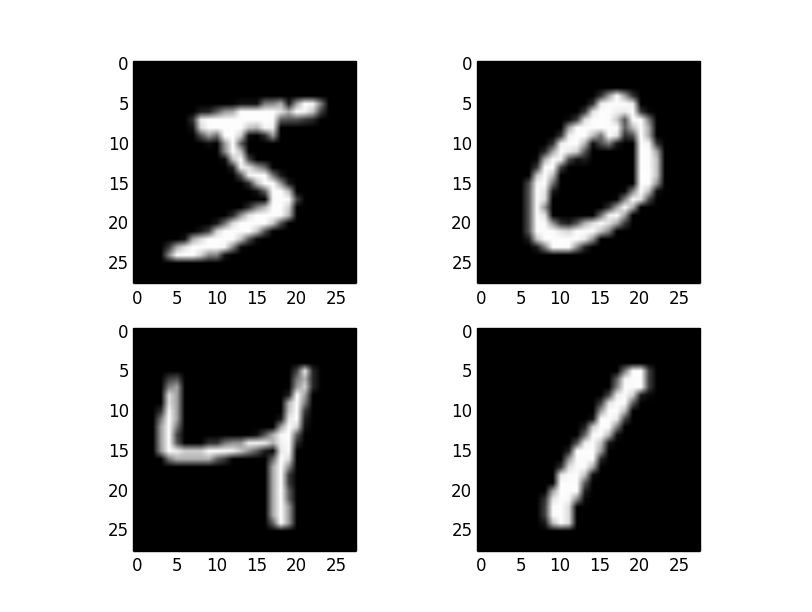
\includegraphics[scale=0.60]{images/mnist.png}
\caption{Historia de las redes neuronales}
\end{figure}\\
No es estrictamentre necesario una red neuronal convolucional para conseguir los mejores resultados con el el dataset MNIST. Mediante una red neuronal sencilla, con una sola capa oculta, podemos alcanzar un ratio de error del 1.74\%. Usaremos este dato como base para comparar mas modelos de redes convolucionales más adelante.\\
Lo primero de todo, como ya hemos visto, es cargar los modulos necesarios, generar una semilla aleatoria (aunque fija), y cargar el dataset.\\
El set de entrenamiento está estructurado como un array tridimensional compuesto de la instancia de la imagen, su ancho y su alto. Para poder utilizarlo con un perceptrón, tenemos que convertir las imagenes en un vector de pixeles. En este caso, las imagenes de 28x28 se convertirán en 748 valores de entrada. Podemos hacer esto facilmente  con la funcion reshape() de NumPy.
\begin{verbatim}
import numpy
from keras.datasets import mnist
from keras.models import Sequential
from keras.layers import Dense
from keras.layers import Dropout
from keras.utils import np_utils

numpy.random.seed(7)

n_pixels = X_train.shape[1] * X_train.shape[2]
X_train = X_train.reshape(X_train.shape[0], n_pixels).astype('float32')
X_test = X_test.reshape(X_test.shape[0], n_pixels).astype('float32')
\end{verbatim}

Los valores van de 0 a 255, en una escala de grises. Cuando trabajamos con modelos de redes neuronales, suele ser buena idea escalar o normalizar los datos de entrada. Para ello, convertiremos estos valores de 0-255 a 0-1.\\
Además, la salida será un entero entre 0 y 9 (ya que como hemos dicho, tenemos 10 clases en las que nuestra imagen puede ser clasificada). Nos encontramos ante un problema de multiclasificación, por lo que será util codificar el vector de enteros en una matriz binaria:
\begin{verbatim}
X_train = X_train / 255
X_test = X_test / 255

y_train = np_utils.to_categorical(y_train)
y_test = np_utils.to_categorical(y_test)
num_classes = y_test.shape[1]
\end{verbatim}

Con todo esto, ya podemos crear el modelo de la red neuronal. En este ejemplo, vamos a diseñar tanto un modelo de red neuronal utilizando un perceptron multicapa, como un modelo convolucional, para ver sus diferencias y rendimientos a la hora de tratar imagenes.\\
\subsubsection{Perceptrón multicapa}
\begin{verbatim}
def perceptron_model():
	model = Sequential()
	model.add(Dense(n_pixels, input_dim=n_pixels, init='normal', activation='relu'))
	model.add(Dense(num_classes, init='normal', activation='softmax'))
	model.compile(loss='categorical_crossentropy', optimizer='adam', metrics=['accuracy'])
	return model
\end{verbatim}
Como podemos observar, se trata de un modelo con una sola capa oculta, con el mismo numero de neuronas que de entradas, es decir, 784. Además, sobre ella se aplica una funcion de activacion rectificadora.\\
En la capa de salida, se usa la funcion de activacion softmax para convertir las salidad en probabilidad, y permitir que se seleccionen una de las 10 clases que el modelo ha de predecir. Como función de perdida, se utiliza la perdida logarítmica (en Keras, categorical\_crossentropy). Por ultimo, para aprender los pesos, se utiliza el algoritmo gradiente descendiente ADAM.\\
\subsubsection{Red convolucional}
\begin{verbatim}
def convolutional_model():
	model = Sequential()
	model.add(Convolution2D(32, 5, 5, border_mode='valid', input_shape=(1, 28, 28), activation='relu'))
	model.add(MaxPooling2D(pool_size=(2, 2)))
	model.add(Dropout(0.2))
	model.add(Flatten())
	model.add(Dense(128, activation='relu'))
	model.add(Dense(num_classes, activation='softmax'))
	model.compile(loss='categorical_crossentropy', optimizer='adam', metrics=['accuracy'])
	return model
	\begin{lstlisting}
\end{verbatim}
Como podemos observar, las redes convolucionales son bastante mas complejas que los perceptrones multicapa. En resumen, nuestro modelo cuenta con las siugientes capas:\\
1. La primera capa es una capa convolucional (Convolution2D). Cuenta con 32 mapeadores, de tamaño 5x5, y una funcion de activación rectificadora. Al ser la capa de entrada, esperará imagenes de la forma [[pixeles][ancho][alto]].
2. Después definiremos una capa de pooling que utilizará la funcion maximo, con un tamaño de 2x2.\\
3. La siguiente capa será regularizadora. Se ha configurado para excluir aleatoreamente el 20\% de las neuronas de la capa para reducir el sobreajuste.\\
4. La siguiente capa convertirá la matriz de 2 dimensiones en un vector, permitiendo asñi que la salida pueda ser procesada por una capa totalmente conectada.\\
5. Después se ha añadido una capa totalmente conectada con 128 neuronas y una funcion de activacion rectificadora.\\
6. Finalmente, la capa tendrá 10 neuronas, una por cada clase, y una funcion de activación softmax para hacer una aproximacion de la probabilidad de que cada entrada se corresponda con cada clase (es decir, con cada numero).
\subsection{Resultados}
Ahora ya podemos ajustar y evaluar los modelos. Estos se ajustán cada 10 ciclos, con actualizaciones cada 200 imagenes. Finalmente, se pinta  el ratio de error de clasificación.
\begin{verbatim}
model = perceptron_model() // model.convolutional_model
model.fit(X_train, y_train, validation_data=(X_test, y_test), nb_epoch=10, batch_size=200, verbose=2)
scores = model.evaluate(X_test, y_test, verbose=0)
print("Baseline Error: %.2f%%" % (100-scores[1]*100))
\end{verbatim}
Ejecutando todo el codigo anterior utilizando el modelo del perceptrón multicapa, veremos la siguiente salida. Como podemos observar, esta red neuronal tiene un ratio de error de 1.74\%.
\begin{verbatim}
Train on 60000 samples, validate on 10000 samples
Epoch 1/10
11s - loss: 0.2791 - acc: 0.9203 - val\_loss: 0.1422 - val\_acc: 0.9583
Epoch 2/10
11s - loss: 0.1121 - acc: 0.9680 - val\_loss: 0.0994 - val\_acc: 0.9697
Epoch 3/10
12s - loss: 0.0724 - acc: 0.9790 - val\_loss: 0.0786 - val\_acc: 0.9748
...
Epoch 8/10
12s - loss: 0.0149 - acc: 0.9967 - val\_loss: 0.0628 - val\_acc: 0.9814
Epoch 9/10
12s - loss: 0.0108 - acc: 0.9980 - val\_loss: 0.0595 - val\_acc: 0.9816
Epoch 10/10
12s - loss: 0.0072 - acc: 0.9989 - val\_loss: 0.0577 - val\_acc: 0.9826
Baseline Error: 1.74\%
\end{verbatim}
Sin embargo, si ejecutamos el código utilizando el modelo convolucional, tendriamos un ratio de error de 1.10\%, y la siguiente salida:
\begin{verbatim}
Epoch 1/10
84s - loss: 0.2065 - acc: 0.9370 - val_loss: 0.0759 - val_acc: 0.9756
Epoch 2/10
84s - loss: 0.0644 - acc: 0.9802 - val_loss: 0.0475 - val_acc: 0.9837
Epoch 3/10
89s - loss: 0.0447 - acc: 0.9864 - val_loss: 0.0402 - val_acc: 0.9877
...
Epoch 8/10
89s - loss: 0.0142 - acc: 0.9956 - val_loss: 0.0323 - val_acc: 0.9904
Epoch 9/10
88s - loss: 0.0120 - acc: 0.9961 - val_loss: 0.0343 - val_acc: 0.9901
Epoch 10/10
89s - loss: 0.0108 - acc: 0.9965 - val_loss: 0.0353 - val_acc: 0.9890
Classification Error: 1.10%
\end{verbatim}
Como se puede observar, hemos reducido el error de clasificacion del 1.74\% al 1.10\%. Pero... ¿Podriamos obtener mejores resultados? La respuesta es sí. En este ejemplo, se ha utilizado una red convolucional muy simple. Sin embargo, añadiendo mas capas convolucionales, de pooling y totalmente conectadas, podemos acercanos a una ratios de error muy cercanos al state-of-art actual. Por ejemplo, añadiendo una nueva capa convolucional (model.add(Convolution2D(15, 3, 3, activation='relu')), model.add(MaxPooling2D(pool\_size=(2, 2)))),y una nueva capa totalmente conectada (model.add(Dense(50, activation='relu'))), obtendriamos un ratio de error de  0.89\%.

\section{Generación de textos - Red LSTM}
En este ejemplo, vamos a intentar generar textos que más o menos tengan sentido. Hasta la aparición de las redes neuronales que un ordenador pudiese llevar a cabo esta tarea parecía una idea sacado de una pelicula de ciencia ficción. Sin embargo, con las redes LSTM esto es posible.\\
Las redes neuronales, además de ser usadas para predecir modelos, pueden ser utilizadas para aprender secuencias de un problema y generar mediante estos conocimientos nuevas secuencias. Los modelos que generan nuevas secuencias como este, no solo son utiles para saber como de bien nuestra máquina ha aprendido un problema, si no también para saber mas de un problema en sí mismo.\\
En este ejemplo, vamos a utilizar el libro "La metamorfosis" de Kafka, como dataset para nuestra red neuronal. Esta, va a aprender  las dependencias entre los diferentes caracteres que se vaya encontrando a lo largo del texto, así como las probabilidades de que estos caracteres aparezcan, con el objetivo de generar una nueva secuencia de caracteres, formando así un nuevo texto, y una nueva historia. Sin embargo, este ejemplo también es válido para otro tipo de textos: poemas, código fuente... (siempre que estos se encuentren en codigo ASCII).
\subsection{Aprendiendo secuencias de caracteres}
Primero importaremos las clases que vamos a utilizar en el modelo, y cargaremos el texto convirtiéndolo todo a minúsculas.
\begin{verbatim}
import numpy
from keras.models import Sequential
from keras.layers import Dense
from keras.layers import Dropout
from keras.layers import LSTM
from keras.callbacks import ModelCheckpoint
from keras.utils import np_utils

# load ascii text and covert to lowercase
filename = "metamorfosis.txt"
raw_text = open(filename).read()
raw_text = raw_text.lower()
\end{verbatim}
Una vez cargado el libro en memoria, debemos preparlo para ser tratado por una red neuronal. Una buena idea es convertir los caracteres a numeros enteros. Para ello, primero se identifican todos los caracteres que componen el texto y se asocia un numero a cada uno. Con ello, conseguiremos reducir el numero de caracteres a analizar, ya que también eliminado los repetidos.
\begin{verbatim}
# create mapping of unique chars to integers
chars = sorted(list(set(raw_text)))
char_to_int = dict((c, i) for i, c in enumerate(chars))
\end{verbatim}
El siguiente paso es definir el conjunto de entrenamiento. Se dividirá el texto en conjuntos de caracteres (en este ejemplo 100), para pasarselos como entrada a la red neuronal. El objetivo es que la red prediga el caracter 101. Esto se conseguirá desplazando de 1 en 1 los 100 caracteres seleccionados, permitiendo así que cada caracter sea aprendido por los 100 caracteres que le preceden. Por ejemplo, si hiciesemos divisiones de 5 en 5, y tuviesemos la palabra CAPITULO, las iteraciones serían:
\begin{verbatim}
CAPIT -> U
APITU -> L
PITUL -> O
\end{lstlisting}
Dado que las redes neuronales trabajan con numeros en vez de caracteres, debemos convertir estos caracteres a enteros usando la tabla que generamos anteriormente.
\begin{lstlisting}
# prepare the dataset of input to output pairs encoded as integers
seq_length = 100
dataX = []
dataY = []
for i in range(0, n_chars - seq_length, 1):
	seq_in = raw_text[i:i + seq_length]
	seq_out = raw_text[i + seq_length]
	dataX.append([char_to_int[char] for char in seq_in])
	dataY.append(char_to_int[seq_out])
n_patterns = len(dataX)
print "Total Patterns: ", n_patterns
\end{verbatim}
Si ejecutamos el código hasta este punto, podemos ver el numero de dataset de entrenamiento: 147574\\
Una vez que hemos preparado el dataset, necesitamos tranformalo para que pueda ser usado por Keras. Primero, debemos transformar la lista de entradas (seq\_in) en una secuencia de de la forma [muestra, intervalo de tiempo, característica], esperada por una red LSTM. Después, se necesita escalar los enteros al rango 0-1 para conseguir patrones mas faciles de aprender por la red LSTM que usa la función de activación sigmoide. Finalmente, se convertirán los patrones de salida. Para ello, se representará la salida como una prababilidad de que aparezca cada uno de los 47 diferentes catacteres del vocabulario, en vez de intentar predecir estrictamente el siguiente caracter. Cada valor será convertido a un vector de longitud 47, relleno de 0 menos un 1 que concidirá con la columna de la letra que el patron representa. Por ejemplo, si la letra fuese la C (entero numero 3), la codificacion seróa... [0,0,1,0,0,0,0,0...0]
Esto se consigue mediante las siguientes lineas de codigo.
\begin{verbatim}
# reshape X to be [samples, time steps, features]
X = numpy.reshape(dataX, (n_patterns, seq_length, 1))
# normalize
X = X / float(n_vocab)
# one hot encode the output variable
y = np_utils.to_categorical(dataY)
\end{verbatim}
Una vez que tenemos los datos preparados, es hora de definir nuestra red LSTM. Para este ejemplo, se define una sola capa oculta LSTM con 256 unidades de memoria. En este ejemplo se usa la tecnica de regularización para evitar el sobreajuste conocida como Dropout, con una probabilidad de 20. La capa de salida será una capa Dense usando softmax como función de activación para producir una salida en función de la probabilidad de que aparezca uno de los 47 caracteres.\\
En realidad, podemos observar que el problema es realmente un problema de clasificacion con 47 clases, y por ello se define la funcion de perdida logaritmica cross entropy, y se aplica el algoritmo de optimización ADAM para mejorar la velocidad.
\begin{verbatim}
# define the LSTM model
model = Sequential()
model.add(LSTM(256, input_shape=(X.shape[1], X.shape[2])))
model.add(Dropout(0.2))
model.add(Dense(y.shape[1], activation='softmax'))
model.compile(loss='categorical_crossentropy', optimizer='adam')
\end{verbatim}
En este ejemplo, no estamos interesados en la precisión de la clasificación, ya que creariamos un modelo que predeciría cada caracter del conjunto de entrenamiento perfectamente. En vez de eso, estamos interesados en una generalizacion del dataset que minimice la funcion de perdida. Es decir, estamos buscando un balance entre generalización y sobreajuste.\\
Esta red es lenta de entrenar. Por ello, se ha decidido usar una serie de checkpoints para almacenar todos los pesos de la red en un fichero cada vez que se observe una mejora en la perdida, al final de cada ciclo. Usaremos los mejores pesos (menores perdidas) para generar nuestro modelo en el siguente punto.
\begin{verbatim}
# define the checkpoint
filepath="weights-improvement-{epoch:02d}-{loss:.4f}.hdf5"
checkpoint = ModelCheckpoint(filepath, monitor='loss', verbose=1, save_best_only=True, mode='min')
callbacks_list = [checkpoint]
\end{verbatim}
Por ultimo, ya solo queda ajustar nuestro modelo. Usaremos 20 ciclos y una tamaño de lote de 128 patrones.
\begin{verbatim}
model.fit(X, y, nb_epoch=20, batch_size=128, callbacks=callbacks_list)
\end{verbatim}
Cada vez que ejecutamos el modelo, podemos apreciar que nos encontramos ante diferentes valores. Esto es debido a la naturaleza aleatoria del modelo y a que es dificil elegir una semilla aleatoria para las redes LSTM que reproduzcan los resultados con un 100x100 de exactitud. A pesar de ello, este no es el objetivo del modelo.\\
Una vez ejecutado el script completo, se deben haber generado una serie de archivos checkpoint con los mejores pesos de cada ciclo. Para ejecutar el codigo del siguiente apartado donde ya generaremos nuevas secuencias de caracteres, usaremos los valores del ultimo archivo, ya que son los que tienen un menor valor de perdida.
\subsection{Generando secuencias de caracteres}
Una vez entrenada nuestra red, tenemos que cargar los pesos que hemos calculado anteriormente y hemos guardado en nuestro checkpoint.
\begin{verbatim}
filename = "weights-improvement-19-1.9435.hdf5"
model.load_weights(filename)
model.compile(loss='categorical_crossentropy', optimizer='adam')
\end{verbatim}
Además, tambien tenemos que crear un mapeo inverso de caracteres a enteros para convertir de nuevo los enteros utilizados en la red a caracteres.
\begin{verbatim}
int_to_char = dict((i, c) for i, c in enumerate(chars))
\end{verbatim}
Por último, ya solo queda hacer predicciones. La manera mas simple es iniciar con una secuencia de semillas como entrada, generar el siguiente caracter, después actualizar la secuencia de semillas para añadir el caracter generado al final, y quitar el primer caracter.  Este proceso se repetirá mientras queramos generar nuevos caracteres. Elegiremos un patron aleatorio de entrada como nuestra secuencia de semillas, y pintar los caracteres segun se vayan generando.
\begin{verbatim}
start = numpy.random.randint(0, len(dataX)-1)
pattern = dataX[start]
print "Seed:"
print "\"", ''.join([int_to_char[value] for value in pattern]), "\""

for i in range(1000):
	x = numpy.reshape(pattern, (1, len(pattern), 1))
	x = x / float(n_vocab)
	prediction = model.predict(x, verbose=0)
	index = numpy.argmax(prediction)
	result = int_to_char[index]
	seq_in = [int_to_char[value] for value in pattern]
	sys.stdout.write(result)
	pattern.append(index)
	pattern = pattern[1:len(pattern)]
print "\nDone."
\end{verbatim}
\subsection{Analizando resultados}
Al ejecutar el codigo anterior, nuestro programa genera el siguiente texto:
\begin{verbatim}
R
E
L
L
E
N
A
R
\end{verbatim}
Como podemos ver, los resultados no son perfectos. Hay palabras que si han sido generadas correctamente (como RELLENAR), y otras que sin embargo, no tienen mucho sentido (como RELLENAR).\\
Con diseños mas avanzados, nuestra red reflejaría mejores resultados. Una propuesta de modelo mas avanzado, pero que por tanto, tardaría mas en entrenarse sería por ejemplo la siguiente:
\begin{verbatim}
model = Sequential()
model.add(LSTM(256, input_shape=(X.shape[1], X.shape[2]), return_sequences=True))
model.add(Dropout(0.2))
model.add(LSTM(256))
model.add(Dropout(0.2))
model.add(Dense(y.shape[1], activation='softmax'))
model.compile(loss='categorical_crossentropy', optimizer='adam')
\end{verbatim}
Además, tambien podemos incrementar el numero de ciclos de entrenamiento de 20 a 50, y disminuir el tamaño de lote de 128 a 64 para dar a la red la oportunidad de aprender más.
\begin{verbatim}
model.fit(X, y, nb_epoch=50, batch_size=64, callbacks=callbacks_list)
\end{verbatim}
Además, hay una serie de tecnicas que ayudarían a mejorar nuestro nuevo texto, pero que en este ejemplo no han sido aplicadas. Algunas de ellas son:
\begin{itemize}
\item Predecir menos de 1000 caracteres de salida por semilla
\item Borrar todos los signos de puntuacion y por tanto, del vocabulario del modelo.
\item Añadir mas capas al modelo
\item Reducir el tamaño de lote (el más eficiente seria de 1, pero nuestro modelo tardaría mucho en entrenarse)
\end{itemize}

\chapter{Conclusiones y lineas futuras}
\label{chap:conclusiones}


\newpage \thispagestyle{empty} % P�gina vac�a 

\chapter*{Glosario de acrónimos}
\addcontentsline{toc}{chapter}{Glosario de acrónimos}

\begin{itemize}
\item{\textbf{LSTM}:  Long Short-Term Memory}
\item{\textbf{RNN}:  Recurrent Neural Network}
\item{\textbf{FNN}: Feed-forward Neural Network}

\end{itemize}

\newpage \thispagestyle{empty} % Pagina vacia

\addcontentsline{toc}{chapter}{Bibliografía}    %Agregamos al indice el capitulo de bibliografia


\bibliographystyle{unsrt}   %plain pero ordenado en orden de aparacicion en documento principal
\bibliography{bibliografia}

\appendix   %Indicamos que lo que viene a continuacion son apendices

%\frontmatter %Para poner los anexos en numeros romanos

\chapter{Manual de utilización}
\label{Anexo:manualuso}


\newpage \thispagestyle{empty} % Página vacía 

%\input{anexo_maualprogramador}

%Hoja final en blanco
\newpage \thispagestyle{empty} % Pagina vacia

\end{document}
